\documentclass[letterpaper,12pt,oneside]{book}
\usepackage[top=1in, left=1in, right=1in, bottom=1in]{geometry}
%-----------------------__--------
%https://es.overleaf.com/project/642e50d937469ff17340bdc4
% Tesis UNAM https://tex.stackexchange.com/questions/234265/unam-thesis-title-page-portada-tesis-unam

%\usepackage{parskip} % Add the parskip package


\usepackage{setspace} % Add the setspace package
\setstretch{1.5} % Set line spacing to double

\usepackage{pdfpages}
\usepackage{lipsum}

\usepackage[T1]{fontenc}
\usepackage[utf8]{inputenc}
\usepackage[spanish,es-nodecimaldot,es-tabla]{babel}
\usepackage{graphicx}
\usepackage{tikz}
\usepackage{setspace}


%Subfiguras
\usepackage{caption}
\usepackage{subcaption}

% Para referencias 
\usepackage{hyperref}
\usepackage{apacite}
\usepackage{url}

%\addbibresource{CARDIAC}


\title{E-CARDIAC: La evolución hacia un modelo concurrente y paralelo}

\begin{document}
	\frontmatter
	\pagestyle{plain} % Set page style to "plain" for the front matter
	%\maketitle

    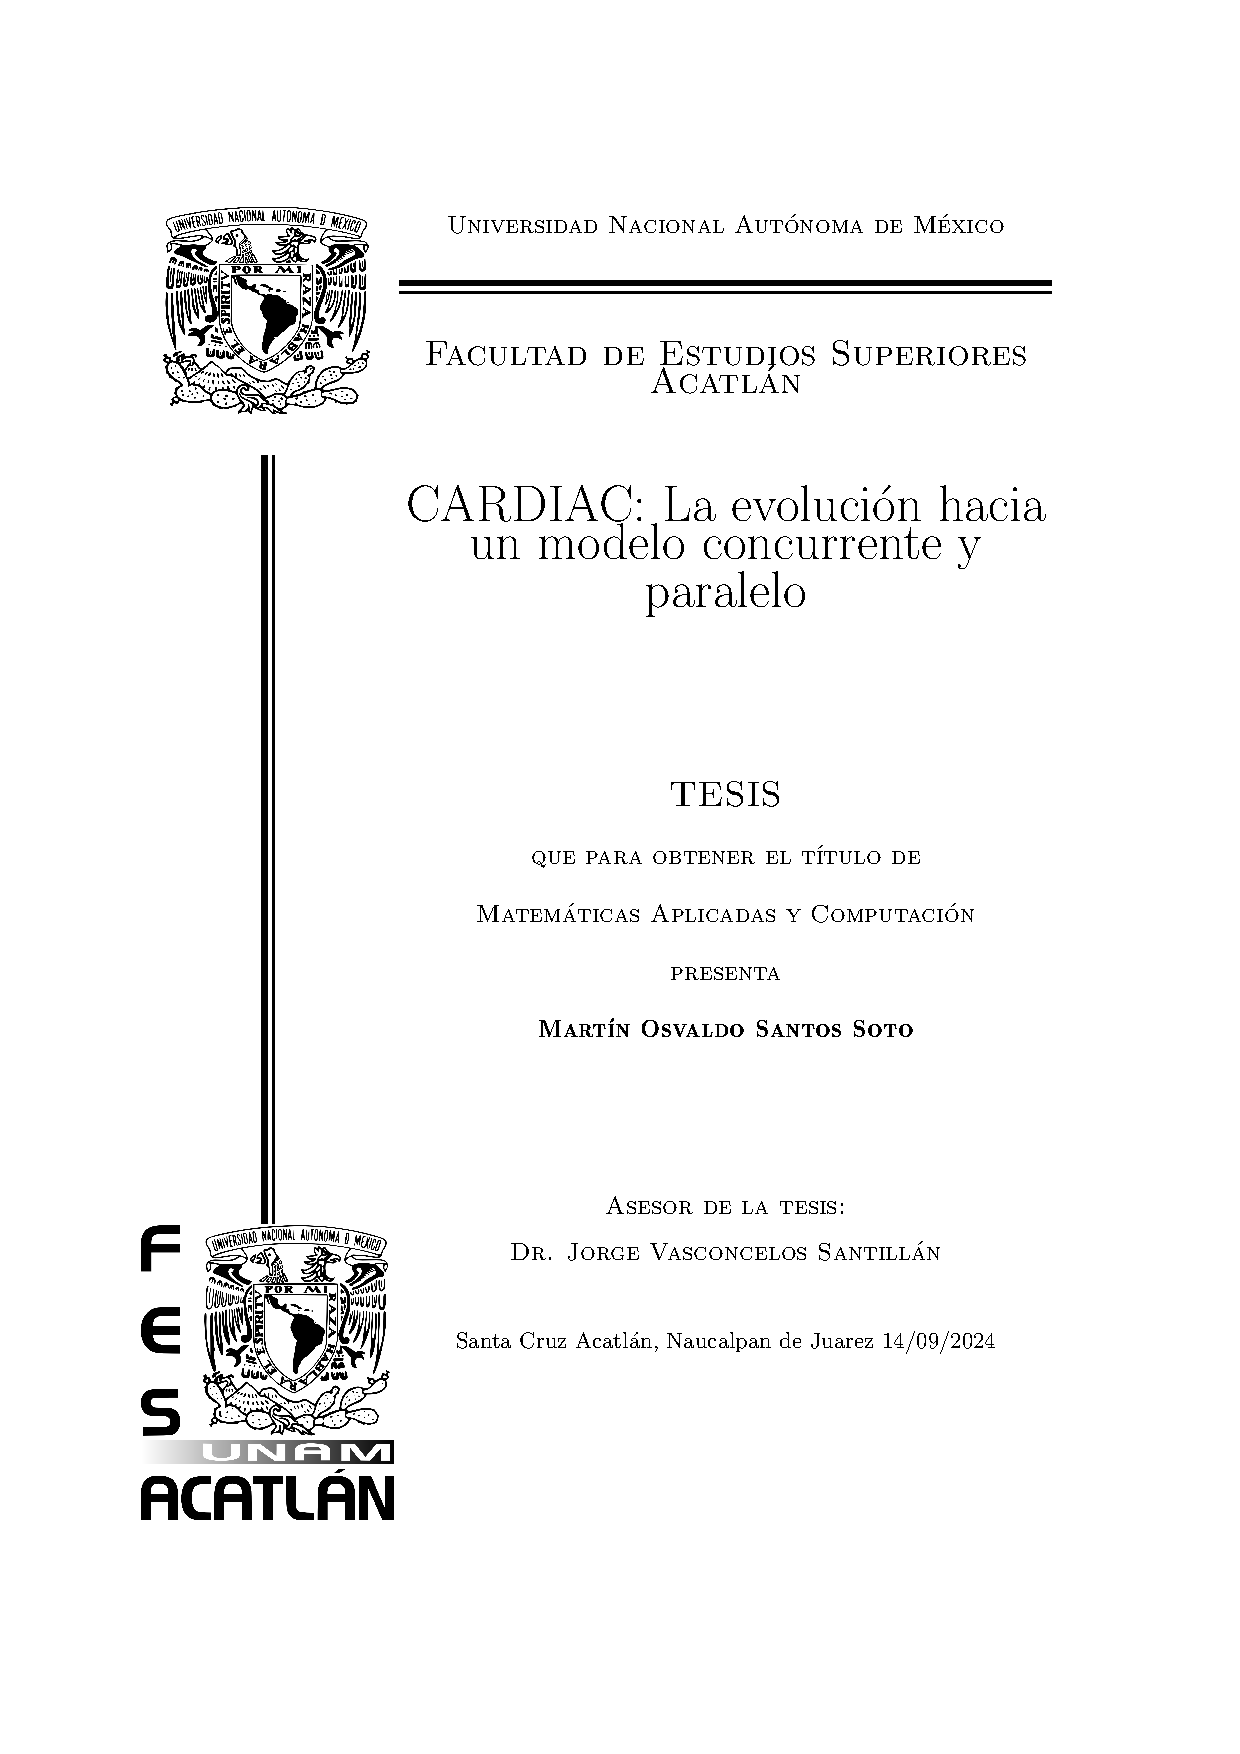
\includepdf{media/cover.pdf}

%---------------------------------
\chapter*{}
\begin{flushright}%
  \emph{``These are fast-moving times, and those who make no effort to understand computers may very well get left behind''}
  
  
  - David W. Hagelbarger, 1968
  %%\thispagestyle{empty}
\end{flushright}

\chapter*{Agradecimientos}
%\spacing{1.5}%\doublespacing

\chapter*{Abstract}

\chapter{Introducción}

	Hoy en día tenemos multitud de aparatos electrónicos que suelen ser llamados computadoras; celulares, laptops, tabletas, relojes inteligentes, y un sin fin más. 
	Estos aparatos suelen ser llamados así dado que son capaces de resolver operaciones aritméticas y lógicas, guardar datos, procesarlos, y recibir instrucciones del 
	usuario, esto siguiendo la definición
	que recoge el diccionario de Oxford\footnote{Usado como fuente dado que la lengua franca de la computación es el inglés.} tiene sentido,
	pero si analizamos más detalladamente el termino ``computadora''  notaremos que el origen de la palabra es anterior a las computadoras
	tal cual las conocemos hoy día, por ejemplo antes de 1950 la palabra ``computadora''  era referida comúnmente a mujeres
	que trabajaban en la NASA y realizaban cálculos manuales, como lo describe el blog \cite{nasa_who_2020} de la NASA dedicado a Katherine Johnson, destacada "computadora humana" que aún con el machismo que se vivía en la época logro ser ampliamente reconocida y ver como esa misma palabra que la había descrito a ella en el pasado
	era usada para describir a potentes maquinas electrónicas de cálculo.

	Si viajamos al pasado remoto notaremos que desde muy temprana edad se buscaba disminuir las tareas repetitivas para los humanos, pasando por el ábaco
	en muchas culturas, hasta maquinas más complejas a partir del siglo XVI, o con técnicas como los logaritmos o las tablas de multiplicar. Esta búsqueda junto
	al desarrollo de otras tecnologías en paralelo permitió la creación de maquinas que podían ir más de allá que automatizar cálculos,
	maquinas de propósito general, que pudieran cambiar su funcionamiento de acuerdo a la interacción con el usuario y resolver
	una multitud de problemas nunca antes pensada\cite{ifrah_universal_2001}. En tal estudio del pasado nos daremos cuenta de la cantidad de sucesos y desarrollos que tuvieron 
	que acontecer para llegar desde automatizaciones muy particulares de cálculos aritméticos hasta las computadoras que conocemos hoy en día. 
	%Sinonimos?
	%%https://www.smithsonianmag.com/science-nature/history-human-computers-180972202/

	Aunque tenemos una remota idea de lo compleja que fue la invención de la computadora no se suele conocer ni siquiera superficialmente
	la forma en que funciona una computadora, el como podemos enviar mensajes de texto mientras escuchamos una canción, si acaso hay algún programa que ejecuta a los 
	demás programas que utilizamos, o incluso si hay un programa que da inicio a todos los procesos de una computadora. Por que al final son temas complejos
	que requieren su tiempo de estudio, lo que no puede suceder es que profesionales o estudiantes de carreras afines a la computación no conozcan estos detalles, y
	es que muchas veces se da por sentado que es conocimiento general y en especializaciones como desarrollo web o arquitectura de software(solo como ejemplo) no se le suele
	prestar mucha atención. Sin embargo el conocimiento, al menos básico, del funcionamiento interno de una computadora es fundamental para saber
	como explotar de mejor manera los recursos de las maquinas que estás utilizando en cualquier disciplina que te desempeñes. Aunado a esto conocer la historia
	es otro punto fundamental,
	te permitirá saber la razón por la cuál ciertos aspectos de las computadoras no han cambiado en 80 años y el por que otros han cambiado o evolucionado
	de manera tan vertiginosa en los últimos años, preparándote también para el futuro y dando el reconocimiento que se merecen a aquellas personas que
	con sus aportes contribuyeron a la revolución que trajo consigo la invención de la computadora.
	
	Estos pensamientos surgieron a lo largo de mi carrera universitaria, pero fue al final de está que decidí abordarlos y empezar este proyecto de investigación
	con el fin de centrar en un mismo texto un repaso histórico de la computación acompañado de una descripción didáctica del funcionamiento de las computadoras
	y su evolución a lo largo de la historia. Pero como la intención tampoco es crear un manual completo de las computadoras y su historia el repaso
	se centrará principalmente en el origen de las computadoras y como funciona, groso modo, una computadora actual. Para esto último me apoyaré
	de \textit{CARDIAC(CARDboard Illustrative Aid to Computation)}, un modelo de computación 
	desarrollado por Bell Labs de la mano de David W. Hagelbarger y Saul Fingerman en 1968\cite{david_hegelbarger_instruction_1968} con la intención, precisamente,
	de hacer más fácil de entender a los alumnos de aquel entonces el como funcionaba una computadora. No fue el único intento, otro que se debe mencionar es
	\textit{Little Man Computer(LMC)} creada por Stuart Madnick y Jhon Donovan del MIT en los años 60, que con un reducido conjunto de instrucciones permitía a los estudiantes 
	probar la ejecución de programas como si estuvieran en una computadora real. Ambos modelos mencionados en \cite{mark_jones_lorenzo_paper_2017}, que
	no puedo dejar de mencionar como una de las lecturas que más me inspiraron en la escritura de está tesis.
	
	El reto con \textit{CARDIAC(CARDboard Illustrative Aid to Computation)} es que fue creado en 1968, por lo que la concurrencia, el paralelismo o
	la inclusión de un sistema operativo no pasaban por la mente de sus creadores dado que aún no eran tan relevantes en la industria estos términos. Así que
	para poder llegar a las computadoras actuales concurrentes, paralelas y con un sistema operativo decidí diseñar una ``evolución'' de CARDIAC que permita
	entender estos conceptos de una forma didáctica, aprovechando las ventajas un modelo que abstrae un sistema complejo en los componentes principales
	que se quieren dar a entender. Aprovechando el contexto histórico se darán las razones por las que cuales cada paso en la evolución de las
	computadoras fue necesario e incluso aveces imparable, manteniendo la atención principalmente en estos 3 conceptos sin desviar la atención en
	muchos otros avances, especialmente de hardware, que son fundamentales pero no el tema central de está tesis.
	 
	Es claro que en todo esté tiempo surgieron otros modelos con la intención de ayudar a los estudiantes a entender el funcionamiento de una computadora, algunos
	de ellos que debo mencionar por su relación con CARDIAC son : \textit{MARIE(Machine Architecture that is Really Intuitive and Easy)} un muy interesante 
	desarrollo presentado en \cite{null_essentials_2003} que se enfoca en los aspectos básicos del funcionamiento al igual que CARDIAC, otro es un desarrollo
	hecho en Argentina alrededor de los años 80 llamado \textit{TIMBA(Terrible Imbecile Machine for Boring Algorithms)} que incluso tenía un lenguaje de programación
	como nos describe el articulo \cite{alvaro_frias_retruco_2022} centrado en dicho lenguaje, por último he de mencionar un desarrollo
	mostrado en el articulo \cite{ajdari_design_2012} que presenta a \textit{Abu-Reiah} un procesador de 8 bits simplificado que incluye un simulador 
	gráfico
	para ayudar a los estudiantes de arquitectura de computación. Mi intención con las mejoras a CARDIAC no es suplir ninguno de los trabajos antes mencionados,
	sino más bien complementarlos con un desarrollo histórico que presente de forma clara, concisa y didáctica 4 aspectos fundamentales en la evolución
	de la computación, la concurrencia, el paralelismo, el uso del sistema operativo y la programación.
	
	
	Más allá del recorrido en la construcción y diseño de modelos ``evolucionados'' de CARDIAC el texto se verá acompañado,
	tal como la clásica CARDIAC distribuida por Bell Labs, con un ``kit'' que incluye un programa que contendrá tres maquinas virtuales\footnote{La emulación de una
	maquina física que virtualiza cada uno de sus componentes, incluido el hardware.}, uno para cada
	modelo de CARDIAC, con la diferencia de que estas maquinas virtuales ya no serán en papel, sino interfaces gráficas para uso en computadoras de escritorio con la idea de 
	que sea fácil para el estudiante
	entender la teoría y practicarla, poder ver como se van ejecutando los programas que ya en una versión paralela o concurrente sería un poco más difícil de ver con una 
	computadora de papel dada la cantidad de información que se tiene que almacenar.
	


\tableofcontents
\listoffigures

\mainmatter

\chapter{Historia de la computación} %


	\section{Breve recorrido por el pasado}
		\subsection{Antecedentes}
		% Maquinas parecidas a las computadoras, que no lo son
		
		Desde que los humanos empezamos a hacer cálculos en el sentido de sumar o restar cantidades representadas por números hemos necesitado de herramientas
		que nos apoyen en la resolución del calculo, y entre más complejo el calculo necesitamos herramientas más complejas. Las
		primeras herramientas para apoyarnos en esto fueron fueron formas de representar los números de formas abstractas, una evolución continua en la abstracción
		de los números permitió a algunas civilizaciones crear artefactos con más potencia de cálculo, como el \textbf{ábaco}; el cuál se ha encontrado
		en diversas civilizaciones en diferentes épocas de la humanidad, el más antiguo del que se tiene registro es el inventado por la civilización
		Sumeria alrededor del año 2700 A.C. Otras civilizaciones siguieron sus desarrollos de manera independiente no solo para llegar a un artefacto
		similar al ábaco, sino para evolucionar su forma de hacer cálculos y la complejidad de estos, como es el caso de los griegos, una de las civilizaciones
		más importantes de nuestro mundo, que dieron un gran aporte al desarrollo de la matemática, tanto que muchos de sus descubrimientos siguen siendo
		enseñados hoy en día, y que por supuesto aumentaron la complejidad en los cálculos aritméticos. Está evolución paralela entre la aritmética que teníamos como humanidad 
		y las herramientas para solucionar esos cálculos
		fue construyendo un camino, o quizá varios, que en ciertos puntos confluyeron en la creación del siguiente hito en la simplificación de la resolución
		de cálculos, la \textbf{calculadora}, y de la misma forma nos llevarían hasta la creación de la primera \textbf{computadora} digital, que posteriormente se convertiría
		en algo mucho más grande y completo de lo que quizá se imaginaba en su creación\cite{ifrah_universal_2001}.
		
		%% Ser más claro para la definición de lo que ingresa a la computadora
		Siguiendo la mencionada evolución es importante mencionar la época en la que surgieron las primeras calculadoras mecánicas, así
		como ciertas herramientas para minimizar el esfuerzo en los cálculos realizados por los usuarios. Es el siglo 17 en Europa occidental,
		saliendo del renacimiento(europeo), en el cuál tienen necesidades más complejas en ciencias exactas y en problemas aplicados, los
		cálculos para la navegación y los astronómicos son ejemplos claros de ello. Por esa razón el descubrimiento de
		los logaritmos por parte de Jhon Napier en 1614 fue uno de los grandes avances en la forma de resolver problemas aritméticos,
		los logaritmos, groso modo, te permiten sustituir multiplicaciones por sumas, lo cuál significa una simplificación enorme
		en la resolución de estas operaciones\cite[p. 24]{oregan_brief_2012}. Pero aún así los cálculos seguían sin ser tan rápidos,
		por lo que se desarrollaron tablas de logaritmos ya calculados que hacían esté proceso más simple; otro avance importante en este
		tiempo fue el desarrollo de dispositivos mecánicos que permitían optimizar ciertos cálculos, \textit{The Gunter Scale} y \textit{The Slide Rule},
		creada la primera por Edmund Gunter y la segunda por William Oughtred como mejora a la primera, fueron dos dispositivos que
		ayudaban en la solución de operaciones aritméticas, de hecho \textit{The Slide Rule}(la regla de cálculo) siguió evolucionando a lo largo de los años para añadir más
		funcionalidades, como el uso de logaritmos, lo que la mantuvo vigente hasta hace relativamente poco tiempo(especialmente en áreas de ingeniería)\cite[p.24 y p. 96]{oregan_brief_2012}.				
		 Un poco más lejos llegarían Blaise Pascal y Wilhelm Gottfried Leibniz con sus inventos, que ya serían calculadoras en forma, Leibniz inventaría la
		\textit{Step Reackoner} o simplemente ``maquina de Leibniz'', que permitía hacer cálculos aritméticos, en el año de 1673, basada en \textit{The Pascaline} o
		\textit{Arithmetic Machine} creada por Pascal en 1642\cite[p.25]{oregan_brief_2012}.Ambas ya podían ser llamadas calculadoras funcionales, aunque ya desde muchos años 
		antes se venía pensando
		en un dispositivo como la calculadora, de hecho Leonardo Da Vinci  dejaría sus planos para construir un dispositivo de calculo(el cual no pudo construir), que
		ingenieros de la época moderna pudieron seguir para crearla\cite{california_state_university_historical_nodate}.
		Podemos notar que las inquietudes por automatizar operaciones estaban
		ya desde antes que la tecnología de su época les permitiera a los inventores llevar a cabo sus planes, pero que a pesar de esto las siguientes
		generaciones siguieron adelante con esas ideas, a veces independientemente y otras usando de base lo que ya existía de antes, para
		continuar con la innovación; este interesante patrón, dónde la teoría avanza más rápido que los desarrollos prácticos, lo veremos de nuevo en el futuro.
		%Slide rule en ingenieria
		
		Aunque las maquinas de Leibniz y Pascal eran calculadoras en forma, su replicación no era tan fácil y tampoco fueron muy populares, pero
		si hay una época dónde replicar maquinas para automatizar procesos va a estar en su auge esa es la \textbf{revolución industrial}. En
		1820 un francés llamado Charles Xavier Thomas de Colmar construyo el \textit{Arithmometer} basándose en la terminología de Leibniz, fue la primer
		calculadora en forma que se vendió masivamente, en los años sucesivos continuo recibiendo mejoras y al final fue toda una inspiración para una multitud de inventores 
		alrededor del mundo\cite[p. 127]{ifrah_universal_2001}.
		
		El antecesor directo de la computadora, y sucesor casi directo del ábaco no sólo había nacido, sino que ya había conseguido llegar a gran parte de
		la población, así que, si ya se había logrado el reto, ¿cuál era el siguiente? ¿hacerla más pequeña? si, más pequeña para que pudiera llegar a más personas,
		más veloz y que pudiera hacerse más fácil el uso para el usuario, al menos esa sería la respuesta general, ¿cual sería la de un visionario? Alguien
		que piensa más allá de las convenciones quizá pensaría un dispositivo que fuera capaz de ir más lejos. Y ese era Charles 
		Babbage,
		un reconocido matemático de su época, miembro fundador de la \textit{Royal Astronomical Society} en 1920, inventor, pionero en la investigación
		de operaciones, alguien muy distinguido en su época sin duda. Para el año de 1821 estaba diseñando su \textit{Differential Engine}, una maquina totalmente mecánica que
		en principio buscaba resolver el problema de precisión que tenían las calculadoras del momento, además de resolver funciones polinómicas de hasta
		grado 6. Lamentablemente no llegaría a ser producida por Charles, en parte por lo difícil(y costoso) que era en la época, y en parte por que Charles ya estaba pensando 
		en algo incluso más innovador; aún así la maquina se logro construir en 1853 por un par de ingenieros suecos que se basaron en los planes de Charles
		\cite[p.201]{oregan_brief_2012}.
		
		Lo que Charles ya estaba pensando, y de hecho en 1833, cuando se dio por terminada la construcción de la \textit{Differential Engine}(por que el maquinista que la 
		construía renuncio), estaba decidido a construir era la  \textit{Analytical Engine}, una maquina capaz de realizar cualquier tarea que pudiera
		ser expresada en notación algebraica  y que disminuía la interacción humana para realizar los cálculos. Era una maquina mucho más compleja, tendría un
		almacenamiento, y un procesador que Charles llamaba \textit{the mill} por que tenía la forma de un molino y era la parte que realizaba las operaciones; además
		contaría con elementos para la entrada y salida de datos usando la idea del \textit{telar de Jacquard}\footnote{ Un telar inventado por el francés Joseph-Marie-	Jacquard en 1804 para poder cambiar los patrones de los tejidos.}, que usaba tarjetas perforadas\footnote{Eran tarjetas de 
		cartón(usualmente) que tenían orificios con los que se representaban patrones, se continuaron usando por mucho tiempo en las computadoras digitales como podemos ver en 
		el vídeo: \emph{Punch Card Programming, \url{https://www.youtube.com/watch?v=KG2M4ttzBnY} }}
		para cambiar los patrones de diseños del telar, Charles pensó en usar estas tarjetas para representar números en ellas para realizar las operaciones
		de la maquina y de está forma podía hacer que su maquina fuese ``programable'', por que de hecho consideraba dos tipos de tarjetas:
		
		\begin{enumerate}
			\item Tarjetas de operación
			\item Tarjetas de datos
		\end{enumerate}
		
		Con está última idea de hecho se puede vislumbrar algo muy parecido a las computadoras con arquitectura Von Neumman, un procesador, almacenamiento interno,
		programas almacenados(en forma de tarjetas de operación y de datos)\cite[p.204]{oregan_brief_2012}. Es más en 1943 Lady Ada Lovelace, una matemática
		que estaba entusiasmada con el trabajo de Charles, realmente brillante, y que escribió un articulo al que 
		nombraría \textit{Notes} al final de una traducción que realizo de un trabajo
		del francés al inglés escrito por Luigi Manebra sobre la \textit{analytical engine}, en las cuales detalla el funcionamiento de la maquina, las cualidades que la 
		hacen diferente a las calculadoras de la época, y
		ejemplos de programas para cálculos realmente complejos como el calculo de los números de Bernoulli(de hecho esté se considera como
		el primer programa de la historia), por supuesto con una cercanía muy alta hacía Charles, como se deja ver en su correspondencia, lo que le permitió realizar un 	
		trabajo muy completo, esté articulo junto con las notas de Ada posteriormente sería publicado
		en al revista \textit{Scientific Memoir} bajo el titulo \textit{Sketch of the analytical engine invented by Charles Babbage}. De los elementos más valioso que nos 
		dejo,fueron por supuesto los programas y los detalles del funcionamiento de la maquina(junto a Manebra) que realizó, pero también su visión sobre el trabajo de 
		Charles, que era un tanto diferente a lo que el mismo consideraba, dado que 
		ella pensaba que la maquina podría actuar sobre otras algo más que números, si se creaban las relaciones correctas entre los números  como representación de algo 
		abstracto para fungir como símbolos se podrían realizar más tareas. Ada consideraba a la maquina analítica como algo muy lejano a las calculadoras de su época,
		y lo era en muchos sentidos, y aunque no fue construida en su tiempo al igual que su predecesora\footnote{Fue construida en 1991 por un equipo en el museo de ciencia de Londres usando los planos de Charles y es exhibida actualmente ahí, probando que Charles tenía razón.}, por sus aportes a la computación
		se le considera como la primer computadora(mecánica) de la historia\cite{eric_kim_ada_1999}.
		
		\begin{figure}
		    \centering
		    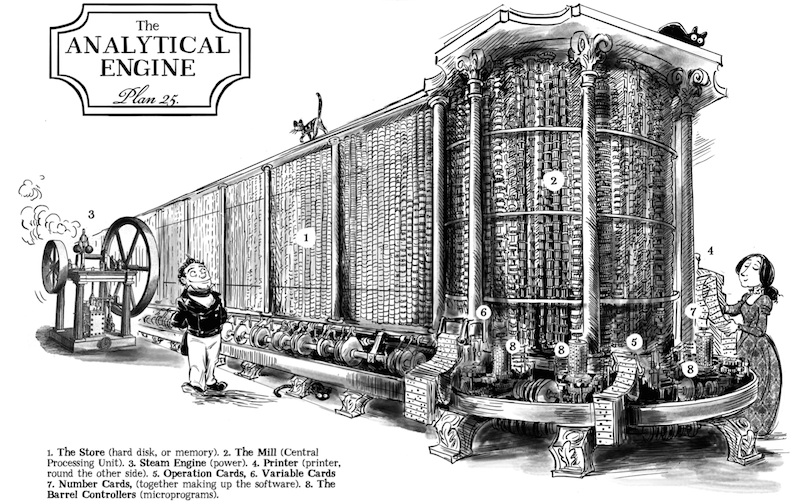
\includegraphics[width=0.7\textwidth]{media/Historia/analyticalEngine1_sydbeypadua.jpg}
		    \caption{Fuente: Sydney Padua (2015), The Analytical Engine.}
	    	\label{fig:analytical_engine}
		\end{figure}
				
		En los años siguientes el avance fue continuo con estás maquinas calculadoras de propósito especifico que fueron mejorando con el paso del tiempo, se desarrollo
		por ejemplo una maquina de censos muy avanzada para su época por el fundador de la empresa hoy conocida como IBM. También la tecnología en general evolucionó,
		la era de la electricidad y lo electromecánico llegó a finales del siglo IX, el invento del tubo de vacío, y también
		avances teóricos que sucedieron, como el álgebra de Boole. Me parece importante hacer notar como no es una sucesión lineal de hechos o descubrimientos
		lo que llevaron a la creación de la computadora digital o de sus predecesoras, sino que el avance en muchas ramas de la ciencia, de la mecánica, y otras
		disciplinas fueron interactuando y creando descubrimientos revolucionarios para su época como lo hemos visto en esté capitulo y como
		se verá en los siguientes. En la siguiente sección analizaremos principalmente ese avance teórico que dio lugar a la evolución de las ``calculadoras'' mecánicas.
		
		% Usar automatas está bien?

		\clearpage		
		
		\subsection{Primeros autómatas}
		% Breve historia de como se fue desarrollando la computación desde los inicios hasta llegar a automatas(1950)
		
		Los avances tecnológicos en las maquinas que automatizan cálculos no pararon, e incluso mejoraron en el siglo 20 con la llegada de la electricidad
		y la electromecánica. Para el año 1913 el matemático Español Leonardo Torres Quevedo desarrollo su \textit{Artimómetro electromecánico}, evitando las
		dificultades que había tenido Babbage con ayuda de la electromecánica y con su gran ingenio pudo llevar a cabo este desarrollo que resolvía diversos
		problemas aritméticos y contaba con una maquina de escribir como entrada. Este no sería el único aporte
		a la computación de Quevedo, otro de los hechos por los que es conocido es por sentar las bases de la \textit{automática} en su \textit{Ensayo sobre automática}, 
		tomando
		la definición de autómata como ``maquina que imita la figura y los movimientos de un ser animado'' Quevedo desarrollo la idea centrado en las posibilidades
		de las maquinas como las calculadoras, pero que pudieran reconocer más objetos, más situaciones y en resolver problemas más difíciles, para así
		quitarles trabajos repetitivos a los humanos. El en su afán de demostrar que su teoría tenía sentido desarrollo un autómata llamado
		\textit{El Ajedrecista} que en su primera versión podía terminar un juego de ajedrez, es decir no podía jugar la partida completa,
		pero podía terminarla\cite{museo_torres_quevedo_ajedrecista_nodate,ifrah_universal_2001}.
		% Cambiar citas para incluir el ensayo de Leonardo Torres Quevedo
		
		Quevedo había lanzado preguntas muy interesantes en su ensayo acerca de los autómatas que se relacionan directamente con la computación, pues cuestiona
		las capacidades de una maquina para hacer algo más que lo que se lograba con una calculadora, aunque por las limitaciones tecnológicas estos cuestionamientos
		eran más teóricas que practicas. Pero, de hecho es justo en la teoría dónde se da el siguiente gran avance en la computación; motivados por \textit{los problemas
		de Hilbert}, una serie de problemas matemáticos que buscaban de dar más rigurosidad a las matemáticas desde el principio del siglo 20, Alan Turing
		y Alonzo Church comenzaron a trabajar por separado en resolver un problema muy particular, el famoso \textit{problema de la parada}, que sin entrar en mucho
		detalle trata sobre saber si todo problema matemático reproducible en un algoritmo puede ser resuelto, si una maquina que está ejecutando el algoritmo
		se detiene con seguridad siempre significa que si puede ser resuelto, siendo un algoritmo una lista de instrucciones ordenadas y finitas que permite solucionar un 
		problema. La resolución
		del problema es muy compleja y no es la idea del texto entrar en esos detalles, pero si dar a entender lo importante que fue para la computación su resolución
		y el trabajo teórico que se hizo.
		
		Se desarrollaron modelos teóricos de maquinas que podían ``computar'' en el sentido más clásico de la palabra, hacer cálculos. Turing trato de crear
		una maquina lo más general posible, de forma que cualquier problema que se pudiera computar en esa ``maquina de propósito general'', sea una calculadora
		o una maquina que resuelve polinomios, a tal maquina la llamo \textit{Maquina Universal de Turing} en su famoso articulo
		\textit{On computable numbers, with an application to the
		Entscheidungsprobkm}(Sobre números computables, con aplicación a el problema de la parada)\footnote{En 1936 se presenta la tesis de Alan Turing y Alonzo Church, con
		aproximaciones distintas a la solución del problema de la parada.}, dando también una definición rigurosa del concepto
		de algoritmo. Un modelo
		totalmente teórico, pero que mostraba todo el potencial de una maquina de propósito general que podía resolver cualquier problema que pudiese ser expresado
		como un algoritmo, pero que no podía resolver todos los problemas aritméticos, por que no hay suficientes algoritmos para representar todos los
		problemas que existen, así que la respuesta al problema de la parada es no, no se pueden resolver todos los problemas matemáticos en base
		a un algoritmo. De está forma se iba creando lo que posteriormente sería conocido como teoría de la computación, un estudio matemáticamente riguroso
		sobre las capacidades de las maquinas de computo que se subdivide en varias ramas, una que nos interesa es la \textit{teoría de la computabilidad}, que estudia
		que algoritmos puede computar una maquina, para llegar a establecer que ciertos problemas son no computables y por ende no son solubles por medio de
		ninguna computadora\cite[p. 272]{ifrah_universal_2001}.
		
		La forma de pensar sobre las maquinas ha evolucionado mucho a esté punto en la historia, la visión ahora es sobre una maquina que de soluciones a problemas que
		puedan ser descritos en forma de algoritmo, y ya no solo soluciones a problemas aritméticos o de funciones matemáticas. Turing y Church
		fueron dos nombres que dieron un salto gigante en está ciencia, que en ese momento aún no existía, de la teoría de la computación. En estos mismos años la evolución
		de en las maquinas continuaba, y en los siguientes años su expansión, causada también por el conflicto armado, no haría más que acelerarse.
		
		\clearpage		
		
		\subsection{Primeras computadoras}
		%1930-1945
		
		Es el momento de hablar de computadoras en forma, maquinas que ya se pueden considerar uniformemente como computadoras para la definición general
		que se tiene de estás. Repasaremos lo sucedido entre el año de 1930 y 1946 dónde por diversas causas, la madurez en el entendimiento de las
		maquinas de cálculo, de la electromecánica y la electricidad, así como necesidades de una mejora tecnológica para enfrentar una de las guerras
		más crueles que ha visto la humanidad, se dieron las condiciones para el desarrollo de la computación. En primera instancia
		como la evolución de las calculadoras, pero que se fue deformando hasta convertirse en más bien maquinas que resolvían problemas específicos.
		
		Como en está parte de la historia está centrada la discusión de cuál fue la primer computadora de la historia es necesario tener una definición
		más clara de lo que entendemos por computadora, y por que ciertas maquinas están en el limbo entre calculadoras o computadoras y otras
		ya son computadoras en un sentido más completo.Empecemos con la definición 
		del diccionario de Oxford, definición que uso dado que es entre Gran Bretaña y Estados Unidos que se da principalmente el desarrollo de las computadoras
		en sus inicios, y por tanto es su lengua franca:
		\begin{enumerate}
			  \item[] \emph{ Definición 1:} Una persona que hace cálculos, especialmente con una maquina de calcular.
			  \item[] \emph{ Definición 2:} Un dispositivo electrónico para guardar y procesar datos, típicamente en forma binaria, de acuerdo a las instrucciones
			  dadas en un programa(conjunto de instrucciones).
		\end{enumerate}
		
		La primera definición, que aún perdura, hace referencia principalmente al significado que tenía antes de 1940. Por que posteriormente, entre 1940 y 1950
		con la aparición de las maquinas electromecánicas o eléctricas se empezó a usar el termino con la connotación que tenemos de el hoy en día. Por ende
		la segunda definición nos interesa más, y que es acorde a muchos libros de computación, como  en \cite{goldstine_computer_1972} Goldstine nos dice lo siguiente 
		acerca de la computadora : ``Es un dispositivo electrónico que puede recibir un conjunto de instrucciones, o un programa,
		y entonces resolver este programa realizando varias operaciones matemáticas en datos numéricos '', a partir de estás definiciones podemos establecer
		4 características fundamentales en una computadora:
		
		\begin{enumerate}
			\item Dispositivo electrónico 
			\item Guarda datos
			\item Procesa datos
			\item Realiza operaciones a partir de un conjunto de instrucciones dadas por el usuario(Entendiendo programa como una forma de algoritmo)
		\end{enumerate}
		
		Todo lo que hace una calculadora lo hace, y con más capacidades, pero hay un punto importante para nuestro estudio, ¿que no sea un dispositivo electrónico es
		necesario para que una maquina que tiene las otras tres características	no sea una computadora? Realmente la mayoría de los autores lo manejan directamente
		como un dispositivo electrónico y no se involucran en la discusión de que es una computadora. Como veremos realmente un dispositivo mecánico o electromecánico
		puede cumplir con el resto de especificaciones, pero dado que su uso fue más bien en el nacimiento de la computación y quedo rápidamente sobrepasado
		por la potencia de los dispositivos electrónicos no se encuentra mucho problema en la definición dada por Goldstine.
		
		%% Pre - Guerra
		
		En está época hubo una gran explosión de desarrollos en cuanto a maquinas que automatizaban cálculos, desde
		aquellas que eran calculadoras muy potentes, algunas que ya entran en la discusión de si son o no computadoras, hasta las que evidentemente lo son.Un ejemplo a 
		resaltar es la \textit{Differential Analiser} creada por Vannevar Bush en 1931 en el M.I.T., uno de los logros más representativos en la historia de las calculadoras
		análogas\footnote{La mayoría de maquinas actuales son digitales por su operación sobre cantidades discretas, mientras que los equipos análogos operan
		sobre cantidades continuas que en versatilidad han quedado superadas por las maquinas digitales.}, dado que desde su inicio se había tenido el problema que eran de un 
		propósito muy especifico, pero está maquina podía resolver una variedad
		más alta de ecuaciones, lo que la convirtió en la primer calculadora análoga multi-propósito\cite[p.158]{ifrah_universal_2001}.
		Otra calculadora realmente llamativa de la época fue la \textit{Complex Number Calculator} creada por		
		Samuel Williams y George Stibitz en los laboratorios Bell, una calculadora electromecánica capaz
		de manejar número complejos, contribución que no fue unica por parte de Stibitz, ya que en Bell Labs desarrollo muchos conceptos relacionados con la
		comunicación y computación, generando así una de las etapas más brillantes para Bell Labs sin duda\cite[p.207]{ifrah_universal_2001}.
		
		
		Precisamente entre estos dos sucesos el Alemán Konrad
		Zuse estaba trabajando en la construcción de prototipos de maquinas que disminuyeran su trabajo como ingeniero; para 1938 había desarrollada la \textit{Z1},
		una calculadora binaria, mecánica, de accionamiento electromecánico y que leía instrucciones de una tarjeta perforada. Para 1939 Konrad llevaría más lejos está idea
		al intentar eliminar la dependencia en las partes mecánicas que eran muy complejas y sustituirlas por relés para funcionar con circuitos eléctricos y
		puertas lógicas(AND,OR,NOT) aprovechando las ideas de George Boole y su álgebra, y de Claude Shannon que introdujo la idea de implementar
		el álgebra booleana mediante relés eléctricos para crear circuitos, está sería la \textit{Z2}.	
		Su siguiente gran trabajo no tardo en llegar, y es por la que es recordado principalmente, la \textbf{Z3}(se puede ver en la figura \ref{fig:zuse_z3}), maquina que fue terminada en 1941; usaba 2600 relés, realizaba aritmética de punto flotante, tenía una ``longitud de palabra''\footnote{En esos años se usaba esa expresión para referirse al tamaño de una variable.} de 22 bits, con un almacenamiento de 64 palabras y los cálculos eran realizados puramente en binario, dado que Zuse lo consideraba más eficiente. Era programable mediante tarjetas
		perforadas y completamente automática, hoy en día es considerada por ciertos autores, como \cite{oregan_brief_2012}, como la primer computadora de programas almacenados de la historia.	
		Aunque dicha atribución podría parecer difícil de hacer
		dado que resulto destruida en 1943 por un bombardeo, fue posteriormente reconstruida y se demostró la capacidad que tenía. De hecho la Z3 es más parecida a las computadoras actuales que computadoras de más renombre como
		la ENIAC, e incluso en 1998 Raúl Rojas probo que la Z3 es Turing Completa, por lo que podemos considerarlo una prueba de que era
		una computadora con la capacidad de computar cualquier problema que pudiera ser expresado como un algoritmo. A pesar de los problemas en Alemania Zuse pudo construir
		una versión más avanzada a la cuál llamo \textit{Z4}, que fue la primer computadora comercial del mundo, introducida al mercado en 1950. Aunque el desconocimiento
		en el resto del mundo fue alto, en los últimos años los museos y los autores le han dado el lugar que merece a uno de los padres de la computación \cite[p.206]{ifrah_universal_2001}.
		
		\begin{figure}
		    \centering
		    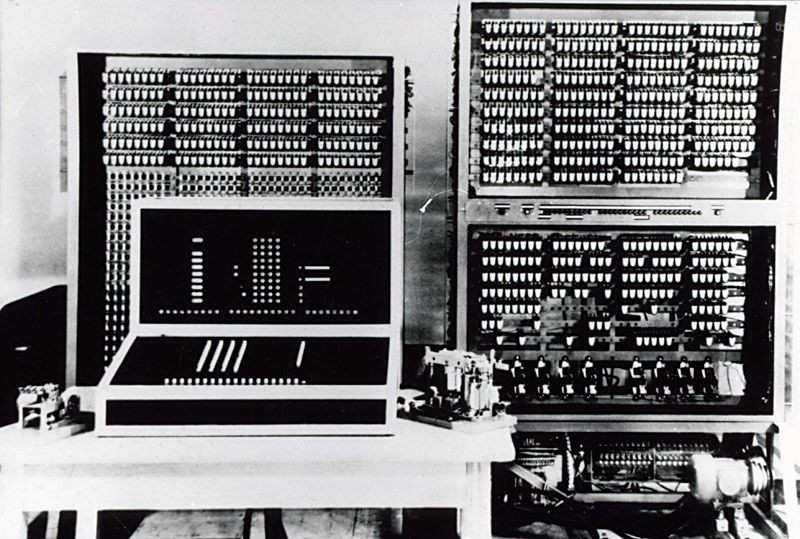
\includegraphics[width=0.7\textwidth]{media/Historia/CHM_computers_1941.zusez3.jpg}
		    \caption{Fuente: Computer History Museum, The Zuse Z3 Computer.}
	    	\label{fig:zuse_z3}
		\end{figure}
		
		
		
		% Guerra
		
		La discusión de cuál fue la primer computadora fue un tema de controversia, tanto que se llevo a tribunales en Estados Unidos dado que los creadores
		de la \textit{ABC} decían que Jhon Mauchly, co-creador de \textit{ENIAC} había visto previamente a la ABC. Finalmente el dictamen fue
		que el concepto de la computadora fue la concepción de diversas ideas por muchas personas, por lo que no era patentable, resolución que tiene mucho sentido
		dada la historia que hemos revisado sobre la creación de las computadoras, muchas mentes han aportado en diversos aspectos a la concepción de lo que hoy
		en día conocemos como computadoras\cite{computer_history_museum_computers_nodate}.
		
		
		Justamente veamos a uno de los implicados en la disputa, que siguió al desarrollo de Zuse, pero sin nada que ver con el. La computadora fue nombrada como 
		\textit{The Atanasoff-Berry Computer(ABC)}, fue construida por el profesor John Vincent Atanasoff 
		en el colegio estatal de Iowa con ayuda de su estudiante Clifford Berry entre 1939 y 1942, tenía un sistema binario para la aritmética, memoria
		para guardad datos, circuitos electrónicos, separación entre datos y programas; era en toda regla una computadora, no programable y de propósito
		especifico. Otro desarrollo en paralelo, pero
		está vez en el M.I.T. fue la \textit{Harvard Mark I}, construida por Howard Aiken y un equipo con apoyo de IBM, destinada a ayudar con cálculos balísticos
		en la segunda guerra mundial, una maquina electromecánica que fue la primera en ser capaz de imprimir tablas matemáticas, algo que Babbage soñó casi un
		siglo atrás\cite[p. 212-218]{ifrah_universal_2001}. Algo interesante a destacar de está maquina es que no tenía las instrucciones y los datos guardados en la misma 
		``memoria'', a diferencia de las que hemos
		visto y lo que será el estándar en cuanto a arquitectura de computadoras; a este tipo de arquitectura se le llamará
		arquitectura Harvard con la llegada de los microprocesadores, una arquitectura que hoy en día empieza a tomar cada vez más relevancia, pero que en su momento
		no fue la arquitectura central del desarrollo de las computadoras\cite{pawson_myth_2022}.
		
		%% No leí el articulo completo, solo el preprint	
		
		%%Tres?
		Después de revisar algunas un tanto desconocidas nos quedan dos que son quizá las famosas computadoras de la época, empezando con 
		\textit{Colossus Mark 1}(figura \ref{fig:colossus}), uno de los grandes aportes que dejo \textit{Bletchley Park}\footnote{Es el nombre de una instalación militar localizada en Buckinghamshire, 	Inglaterra.}, instalación especializada en el trabajo de descifrado de códigos durante la segunda guerra mundial. Con una maquina de descifrado llamada \textit{Bombe}
		lograron desencriptar los mensajes de la famosa maquina enigma, pero con el avance de la guerra se encontraron con un problema aún mayor, la maquina
		\textit{Lorenz SZ40/42} que tenía una codificación de muy alta calidad y se usaba unicamente para los mensajes más importantes en la armada alemana. Para
		descifrar estos códigos es que entra en escena Tommy Flowers diseñando una maquina semi programable que usaba tubos de vacío, lo que la hacía
		relativamente veloz para la época, logrando realizar
		una cantidad ingente de cálculos matemáticos con el fin de descifrar los mensajes que usaban la codificación Lorenz; estando disponible a principios de 1944, y
		su segunda versión unos meses después. Dado su uso militar su existencia se mantuvo
		en alto secreto por orden del gobierno hasta los años 70, hoy en día se conserva una replica de la maquina en el museo de Bletchley Park\cite[p.39]{oregan_brief_2012}.
		
		\begin{figure}
		    \centering
		    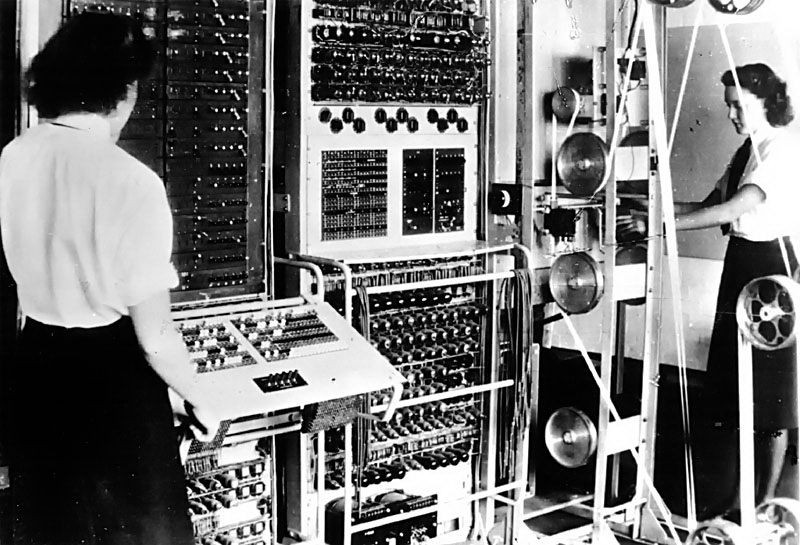
\includegraphics[width=0.7\textwidth]{media/Historia/CHM_computers_1944.colossus.jpg}
		    \caption{Fuente: Computer History Museum, Colossus Mark 1.}
	    	\label{fig:colossus}
		\end{figure}
		
		Prácticamente en paralelo se estaba desarrollando
		en estados unidos una computadora electrónica digital con propósitos militares, centrada en realizar cálculos de artillería para el gobierno,
		\textit{ENIAC ( Electronical Numerical Integrator and Computer)}, computadora construida por John Mauchly, J. Presper Eckert y un equipo, en
		el que se encontraba como consejero externo Jhon von Neumann, en
		\textit{the Moore School of Electrical Engineering of the Univeristy of Pennsylvania}, la cuál a pesar de ser de propósito especifico
		al ser programable se le considera una de las primeras computadoras de propósito general. Su programación era muy compleja, requería de mover o reordenar
		interruptores manualmente e ingresar la información por medio de tarjetas perforadas, 
		lo cuál era realmente tedioso y tardaba demasiado tiempo, si además le sumamos que  los tubos de vacío que usaba no eran muy confiables, puesto que estos explotaban 	
		fácilmente, tenemos una maquina que no era muy confiable y era bastante lenta de programar. Aún así los ingenieros involucrados encontraron la forma de reducir
		las explosiones de los tubos al no  seguido y no hay que perder de vista que lograba reducir el tiempo de procesamiento de horas a segundos en muchos 
		cálculos, un salto enorme en la computación sin duda\cite{ifrah_universal_2001}.
		
		%% Post- Guerra
		
		Fue precisamente en la segunda guerra mundial dónde se dieron los avances más importantes en la historia de la computación, dónde se cambio la forma de
		pensar en maquinas que resolvían cálculos aritméticos a resolver problemas más avanzados, descifra-miento de códigos, calculo de trayectoria para
		misiles y demás tareas propias de una guerra. La necesidad del avance tecnológico llevo a estos desarrollos a su cúspide, pero con el final de
		la guerra los desarrollos no pararon, sino que se incrementaron, y el pensamiento sobre una computadora de propósito general se veía
		presente en las mentes de los científicos que habían impulsado y seguían impulsando los desarrollos de maquinas cada vez más potentes.
		

		En 1946, con la segunda guerra mundial terminada Arthur Bucks, Herman Goldstein y Jhon Von Neumann nos describen en el prefacio de \cite{randell_preliminary_1982}, 
		hacen
		un primer ensayo para sintetizar las ideas que hay sobre estos dispositivos electrónicos, tener una imagen de la situación en la que estaban y
		presentar como los problemas matemáticos podían ser ahora codificados en un lenguaje que la maquina entendiera. Es en esté documento dónde
		se establece por primera vez la arquitectura de una computadora con  \textit{programas almacenados}, concepto fundamental y que hasta hoy
		en día la mayor parte de las computadoras usa. Notaremos que en el titulo de su ensayo no usan en ningún momento la palabra computadora, y
		es que para la época lo que tenían era un dispositivo de computo electrónico, como hemos venido leyendo el uso generalizado de la palabra computadora
		se daría durante el mismo desarrollo de estás. De hecho von Neumann escribiría otro reporte un poco antes llamado \textit{First Draft of a Report on the EDVAC}
		dado que se había unido a Eckert y Mauchly en el desarrollo de
		\textit{EDVAC(Electronic Discrete Variable Automatic Calculator)}, en tal reporte se detalla el diseño de un sistema de computación digital, automático
		y de alta velocidad, fue uno de los textos que marcaron la época y sirvió de inspiración a otros como Maurice Wilkes para el desarrollo de su propia
		computadora con programas almacenados, la \textit{EDSAC(Electronic Display Storage Automatic Computer)}, la cuál tuvo avances muy relevantes que se
		comentaran en capítulos posteriores. La construcción de \textit{EDVAC} tenía la intención de mejorar dónde \textit{ENIAC} fallaba,
		uno fundamental que estaba construida con una arquitectura de programas almacenados, es decir que no se necesitaba reconectar para
		poder ejecutar otra tarea, lo que a su vez ayudaba reducir los errores y facilitaba su programación; se empezó a construir en 1946 y comenzó a operar en 
		1951\cite[p. 45]{oregan_brief_2012}.
		
		Otro de los desarrollos que continuo al final de la guerra, o para ser más preciso, empezó al final de la guerra es el desarrollo de una computadora
		de propósito general en Manchester. Es en Inglaterra con Manchester como uno de sus principales centros
		académicos, en dónde Tom Kilburn y Frederick Williams desarrollaron la primer computadora completamente electrónica, digital, y con programas almacenados;
		en 1948 se culmino la creación de la llamada \textit{Manchester Small Scale Experimental Computer}, mejor conocida como \textit{Baby}
		porque era más pequeña de lo común en la época. Está computadora era más bien un prototipo que después extenderían en la conocida \textit{Manchester Mark I}; de hecho
		ganaría tanta notoriedad por sus avances que una compañía británica
		llamada `` \textit{Ferranti Ltd.}'' se asocio con Kilburn y Williams para comercializar una computadora basada en la que ellos habían construido,
		está llevó el nombre  de \textbf{Ferranti Mark 1} y fue la primer computadora electrónica de propósito general comercializada, la cuál fue liberada
		en Febrero de 1951, poco antes de la \textbf{UNIVAC}, que fue liberada en marzo de 1951\cite[p. 36]{oregan_brief_2012}.
		

		%% Costos de la ferranti		
		
		
		Precisamente para cerrar está época está quizá una de las más recordadas, creada también por Mauchly y Eckert tenemos a la muy conocida	
		\textit{UNIVAC UNIversal Automatic Computer}(figura \ref{fig:univac1}), diseñada como evolución de su propio desarrollo  anterior
		\textit{BINAC (BINary AutomaticComputer(1949)}, la cual erá la primer computadora electrónica con programas almacenados(en EEUU), que basaba su diseño
		a su vez en \textit{EDVAC}.
		Era ya una computadora con programas almacenados como lo venían siendo la mayoría de la época, la decisión no es casualidad, las
		ventajas al momento de escribir instrucciones para estas son muy altas y marcaron un punto de inflexión para el desarrollo de las computadoras,
		el aporte de los programas almacenados puede ser algo simple pero tan importante y revolucionario que se mantiene vigente aún hoy en día. Incluía un teclado y una 
		consola para escribir, era una computadora de negocios realmente, que
		fue entregada la oficina de censos en marzo de 1951(en su versión 1) y se mantendría en comercialización para buscar otros vendedores, aunque no era tan fácil 
		vender una maquina
		tan grande tenía usos muy específicos y quienes podían pagar más de un millón de dólares por ella eran muy pocos; sus compradores en su mayoría
		eran departamentos del gobierno de Estados Unidos como el \textit{U.S. Air Force}, \textit{U.S. Steel} o \textit{U.S. Navy} que son algunos de los departamentos que
		compraron la UNIVAC para su uso además del departamento de censos\cite[p.43]{oregan_brief_2012}.
		
		
		\begin{figure}
		    \centering
		    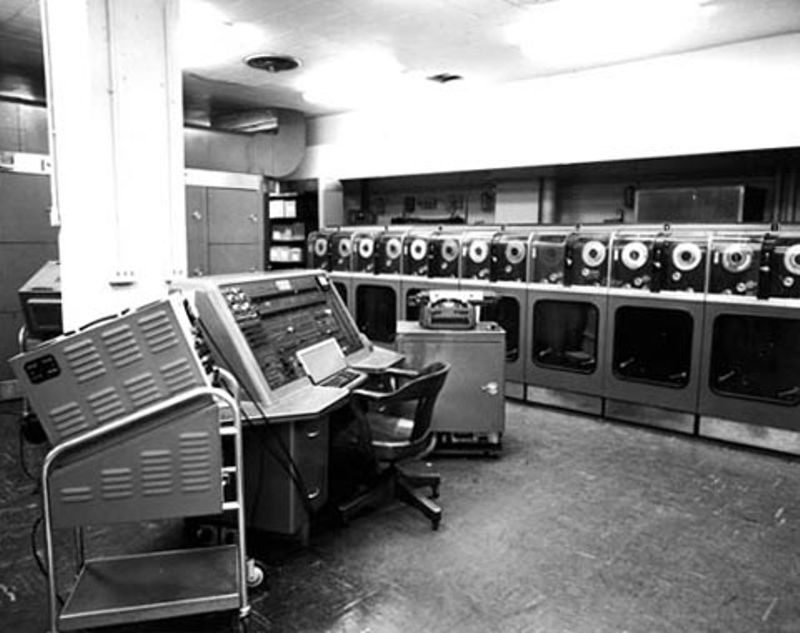
\includegraphics[width=0.7\textwidth]{media/Historia/CHM_computers_1951.univacI.jpg}
		    \caption{Fuente: Computer History Museum, UNIVAC 1.}
	    	\label{fig:univac1}
		\end{figure}
		
		
		% Avance a las siguientes computadoras y la era del Big Iron
		
		Como podemos notar también en la línea de tiempo el desarrollo de computadoras sufrió un crecimiento muy alto, en menos de 20 años se paso de apenas tener la idea
		de una calculadora muy potente a la idea de maquinas completamente electrónicas que resolvían cualquier problema
		que pudiera ser descrito como un algoritmo. Pero aunque el desarrollo tanto en hardware como en software crecía de manera impresionante en
		estos años, para la gente normal las computadoras seguían siendo artefactos muy lejanos, lo cuál es entendible, puesto que
		muy pocas personas en el mundo tenían acceso a una computadora por mucho que sus desarrollos hubieran aumentado. Pero con el tiempo las computadoras
		dejarían ese aspecto de equipos muy especializados sólo para el uso de grandes corporaciones y oficinas del gobierno, una situación fundamental
		para que esto ocurriera fue que los desarrollos dejaron de ser gubernamentales(en EEUU) y empezaron a ser privados con el fin de la segunda guerra mundial.
		De está forma los diseñadores de las computadoras del gobierno empezaron a crear sus propias compañías, como Mauchly y Eckert
		con \textit{Eckert-Mauchly Computer Corporation (EMCC)} o asociarse con otras empresas o bien seguir trabajando de lleno con una compañía de tecnología como
		hizo Aiken en IBM pero para desarrollos comerciales. Esto trajo como resultado la búsqueda de comercializar estos aparatos cada vez más, por lo que tenían que ampliar 
		el mercado y no sólo
		se podían quedar con las maquinas hechas para oficinas gubernamentales, debían llegar a las personas.
		
		%% Imagen comparando los tubos de vacío y las de transistores
		
		\clearpage
		
		\subsection{Expansión de las computadoras: The Big Iron Era}
		
		%% Programación
		
		De acuerdo a \cite{tanenbaum_modern_2002} tenemos 4 generaciones de computadoras, la primera y que revisamos en la sección anterior se caracteriza
		por usar tubos de vacío como conductores eléctricos, lo cuál nos da computadoras gigantes con una alta tendencia al error. La siguiente es caracterizada
		por la invención del \textbf{transistor}\footnote{Un semiconductor que mejoraba en confiabilidad, rapidez y potencia lo que hacían los tubos de vacío y los relés} lo que permitió computadoras más confiables y más pequeñas, los conocidos \textit{mainfraimes}. La
		tercera generación fue la del \textbf{circuito integrado}, que podía juntar cientos de transistores en un espacio realmente pequeño, lo que permitió
		la creación de las famosas \textbf{minicomputadoras}, computadoras del tamaño de un refrigerador pero que en comparación a sus contemporáneas eran realmente
		pequeñas. Por último tenemos la cuarta generación, la generación del \textbf{microprocesador}, que básicamente llevaba toda la parte operativa de la computadora
		a un pequeño dispositivo electrónico que tenía más potencia que varias minicomputadoras juntas.
		
		\begin{itemize}
			\item Primera generación (1945-1955) Tubos de vacío
			\item Segunda generación (1955-1965) Transistores
			\item Tercera generación (1965-1980) Circuitos integrados
			\item Cuarta generación (1980-Presente) Microprocesadores
		\end{itemize}
		
		En la sección anterior nos ubicamos prácticamente en su totalidad en la primera generación y unas décadas antes, para está sección repasaremos algunos
		de los avances fundamentales en la computación, pero principalmente algunas computadoras que aparecieron y su impacto. En la primer y segunda generación es dónde
		se da realmente el avance en cuanto a lenguajes de programación, sistemas operativos, los diversos paradigmas de programación y la
		forma de usar las computadoras,
		por lo que esos temas se dejaran para secciones independientes más adelante para darles un espacio propio.
		
		%% Comentar las principales computadoras de está epoca
		
		A finales de 1954 IBM estrenaba su primer computadora producida en masa, la \textit{IBM 650}, vendiendo alrededor de 450 en ese año y siendo una
		de las últimas grandes computadoras que usaban tubos de vacío. Por que desde principios de los años 50 se dio a conocer el desarrollo del \textbf{transistor}
		por parte de tres inventores en Bell Labs(Shockley, Bardeen and Brattan), esté invento permitía que diseñar circuitos eléctricos para las
		computadoras remplazando los (muy poco confiables) tubos de vacío por estos nuevos semi-conductores con los que podían representar los números binarios
		0 y 1 a través de cargas eléctricas y crear circuitos lógicos más complejos al unirlos. Dado que eran más confiables, duraderos y eficientes, los costos
		y tamaños de las computadoras se redujeron considerablemente, está la era de los mainframes, computadoras del tamaño
		de una habitación con más potencia que las de la primera generación y con un equipo especializado para usarlas; sólo grandes compañías, universidades o
		el gobierno podían pagar los millones que valían\cite{oregan_brief_2012,tanenbaum_modern_2002}.
		
		\begin{figure}
		    \centering
		    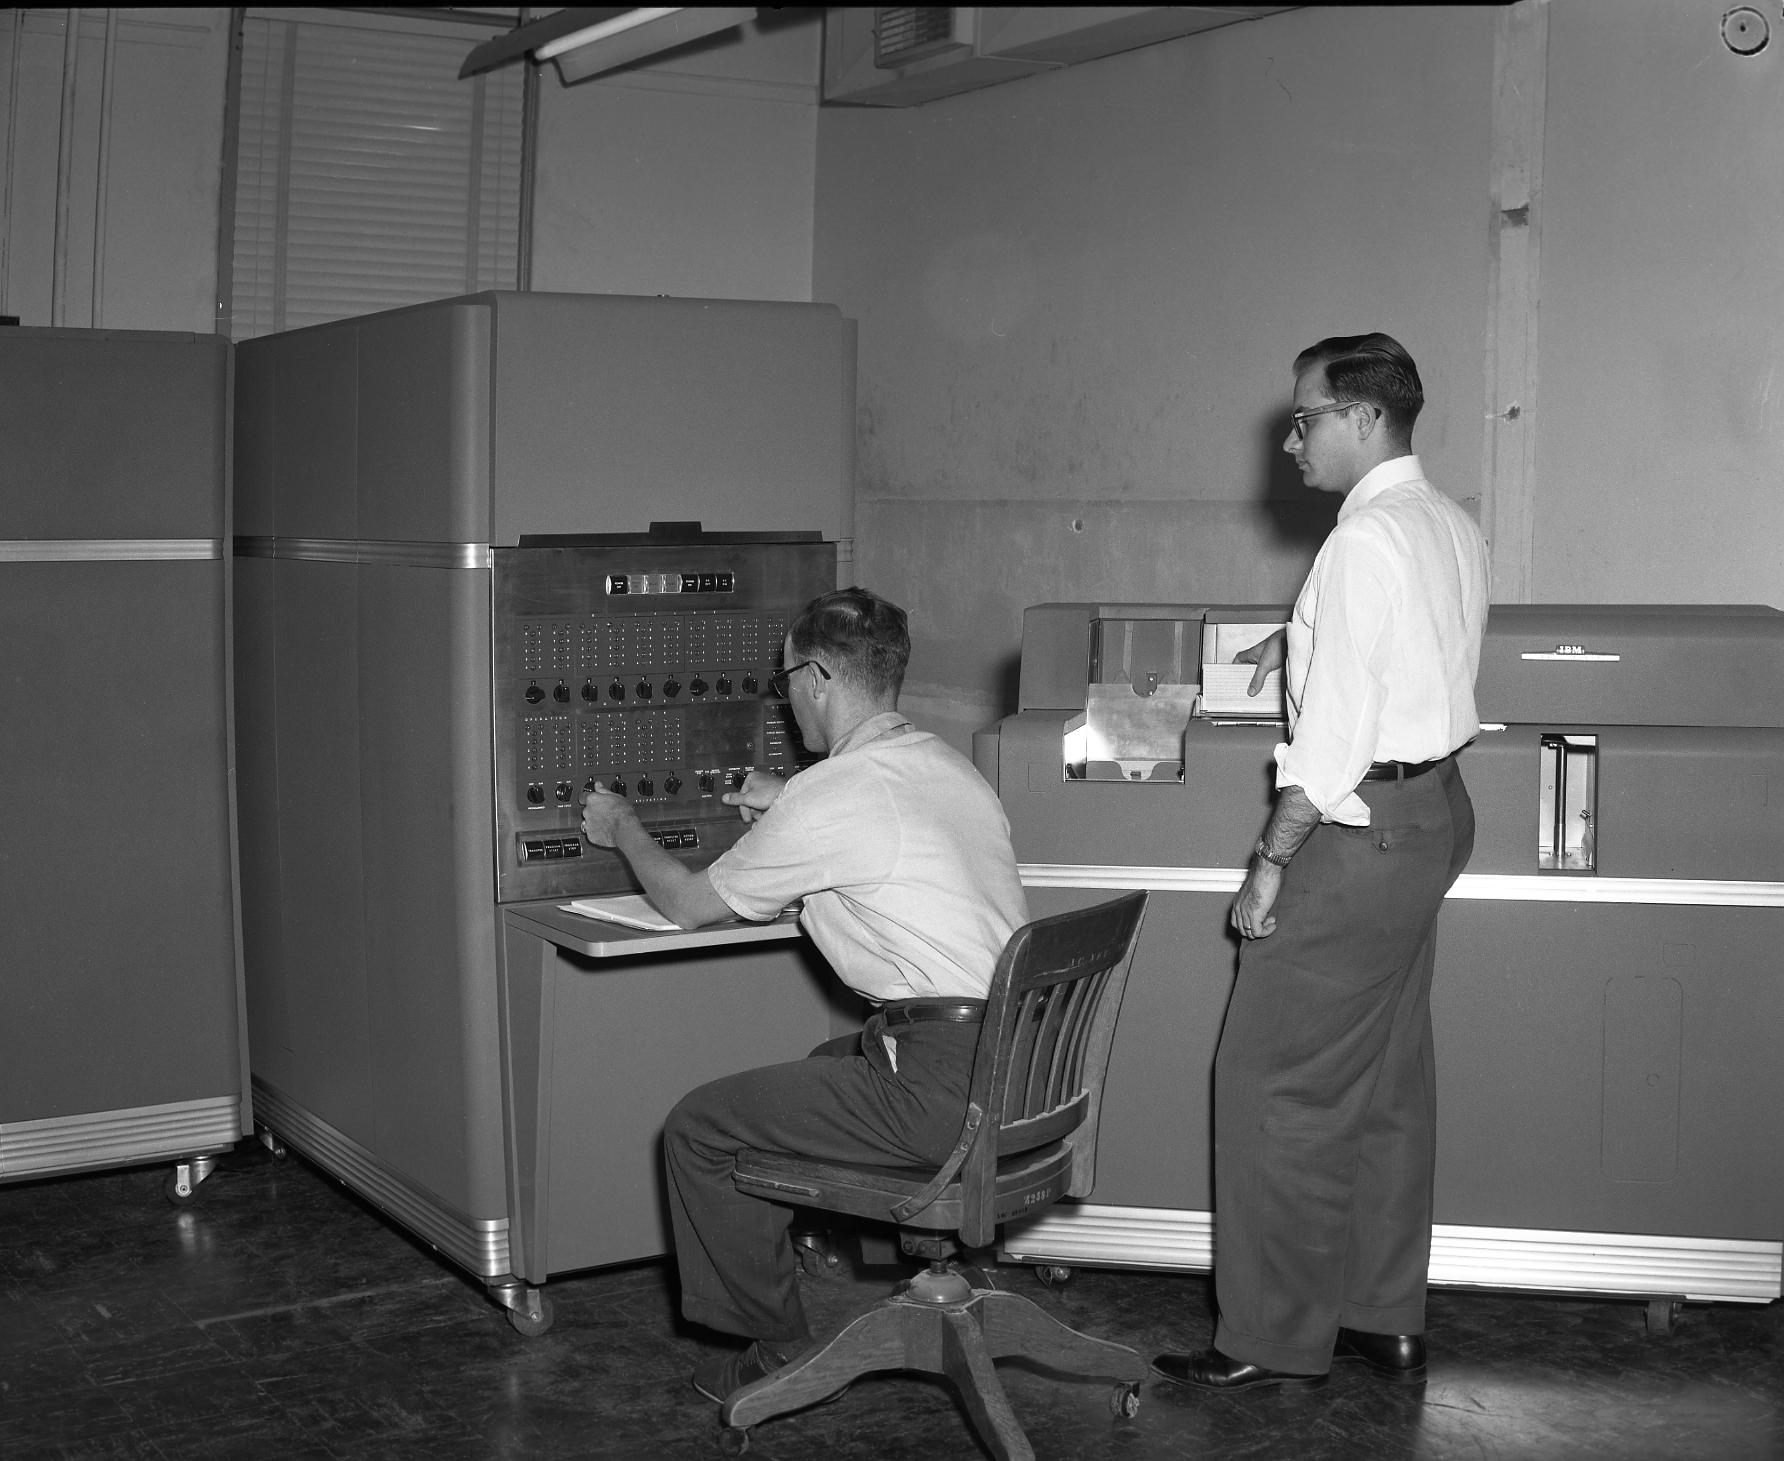
\includegraphics[width=0.7\textwidth]{media/Historia/Wikipedia_IBM_650_at_Texas_A&M.jpeg}
		    \caption{Fuente: ArnoldReinhold - Flickr, IBM 650 en Texas A\&M University.} %% Wikipedia hhttps://en.wikipedia.org/wiki/IBM_650#/media/File:IBM_650_at_Texas_A&M.jpg
	    	\label{fig:ibm650}
		\end{figure}

		%% Insertar imagenes de tubos de vacío vs transistores o computadoras			
		
		Una de las primeras computadoras en usar transistores fue la \textit{PDP-1 (Programable Data Processor)}(1959) desarrollada por \textit{Digital Corporation}, usaba
		2,700 transistores y es muy recordada por que unos estudiantes del MIT escribieron el primer video juego para computadora justo para está misma, el famoso
		\textit{Space War!}. Fue todo un éxito para la empresa que en los siguientes años continuaría teniendo relevancia en el mundo de la computación
		por su continua innovación. Pero IBM siempre va por delante, al menos en esa época, unos años antes, en 1957 introduce la \textit{IBM 608} su primer ordenador
		que usaba transistores en lugar de tubos de vacío, un año después siguió la \textit{7090} que era una maquina especializada para negocios. Y por si fuera poco
		en 1961 estrenarían el tope de su serie 7000, la llamada \textit{IBM 7030 Stretch}, realmente veloz y que representaba la los avances más grandes
		que tenía IBM en ese momento\cite{oregan_brief_2012,computer_history_museum_computers_nodate}.
		
		\begin{figure}
		    \centering
		    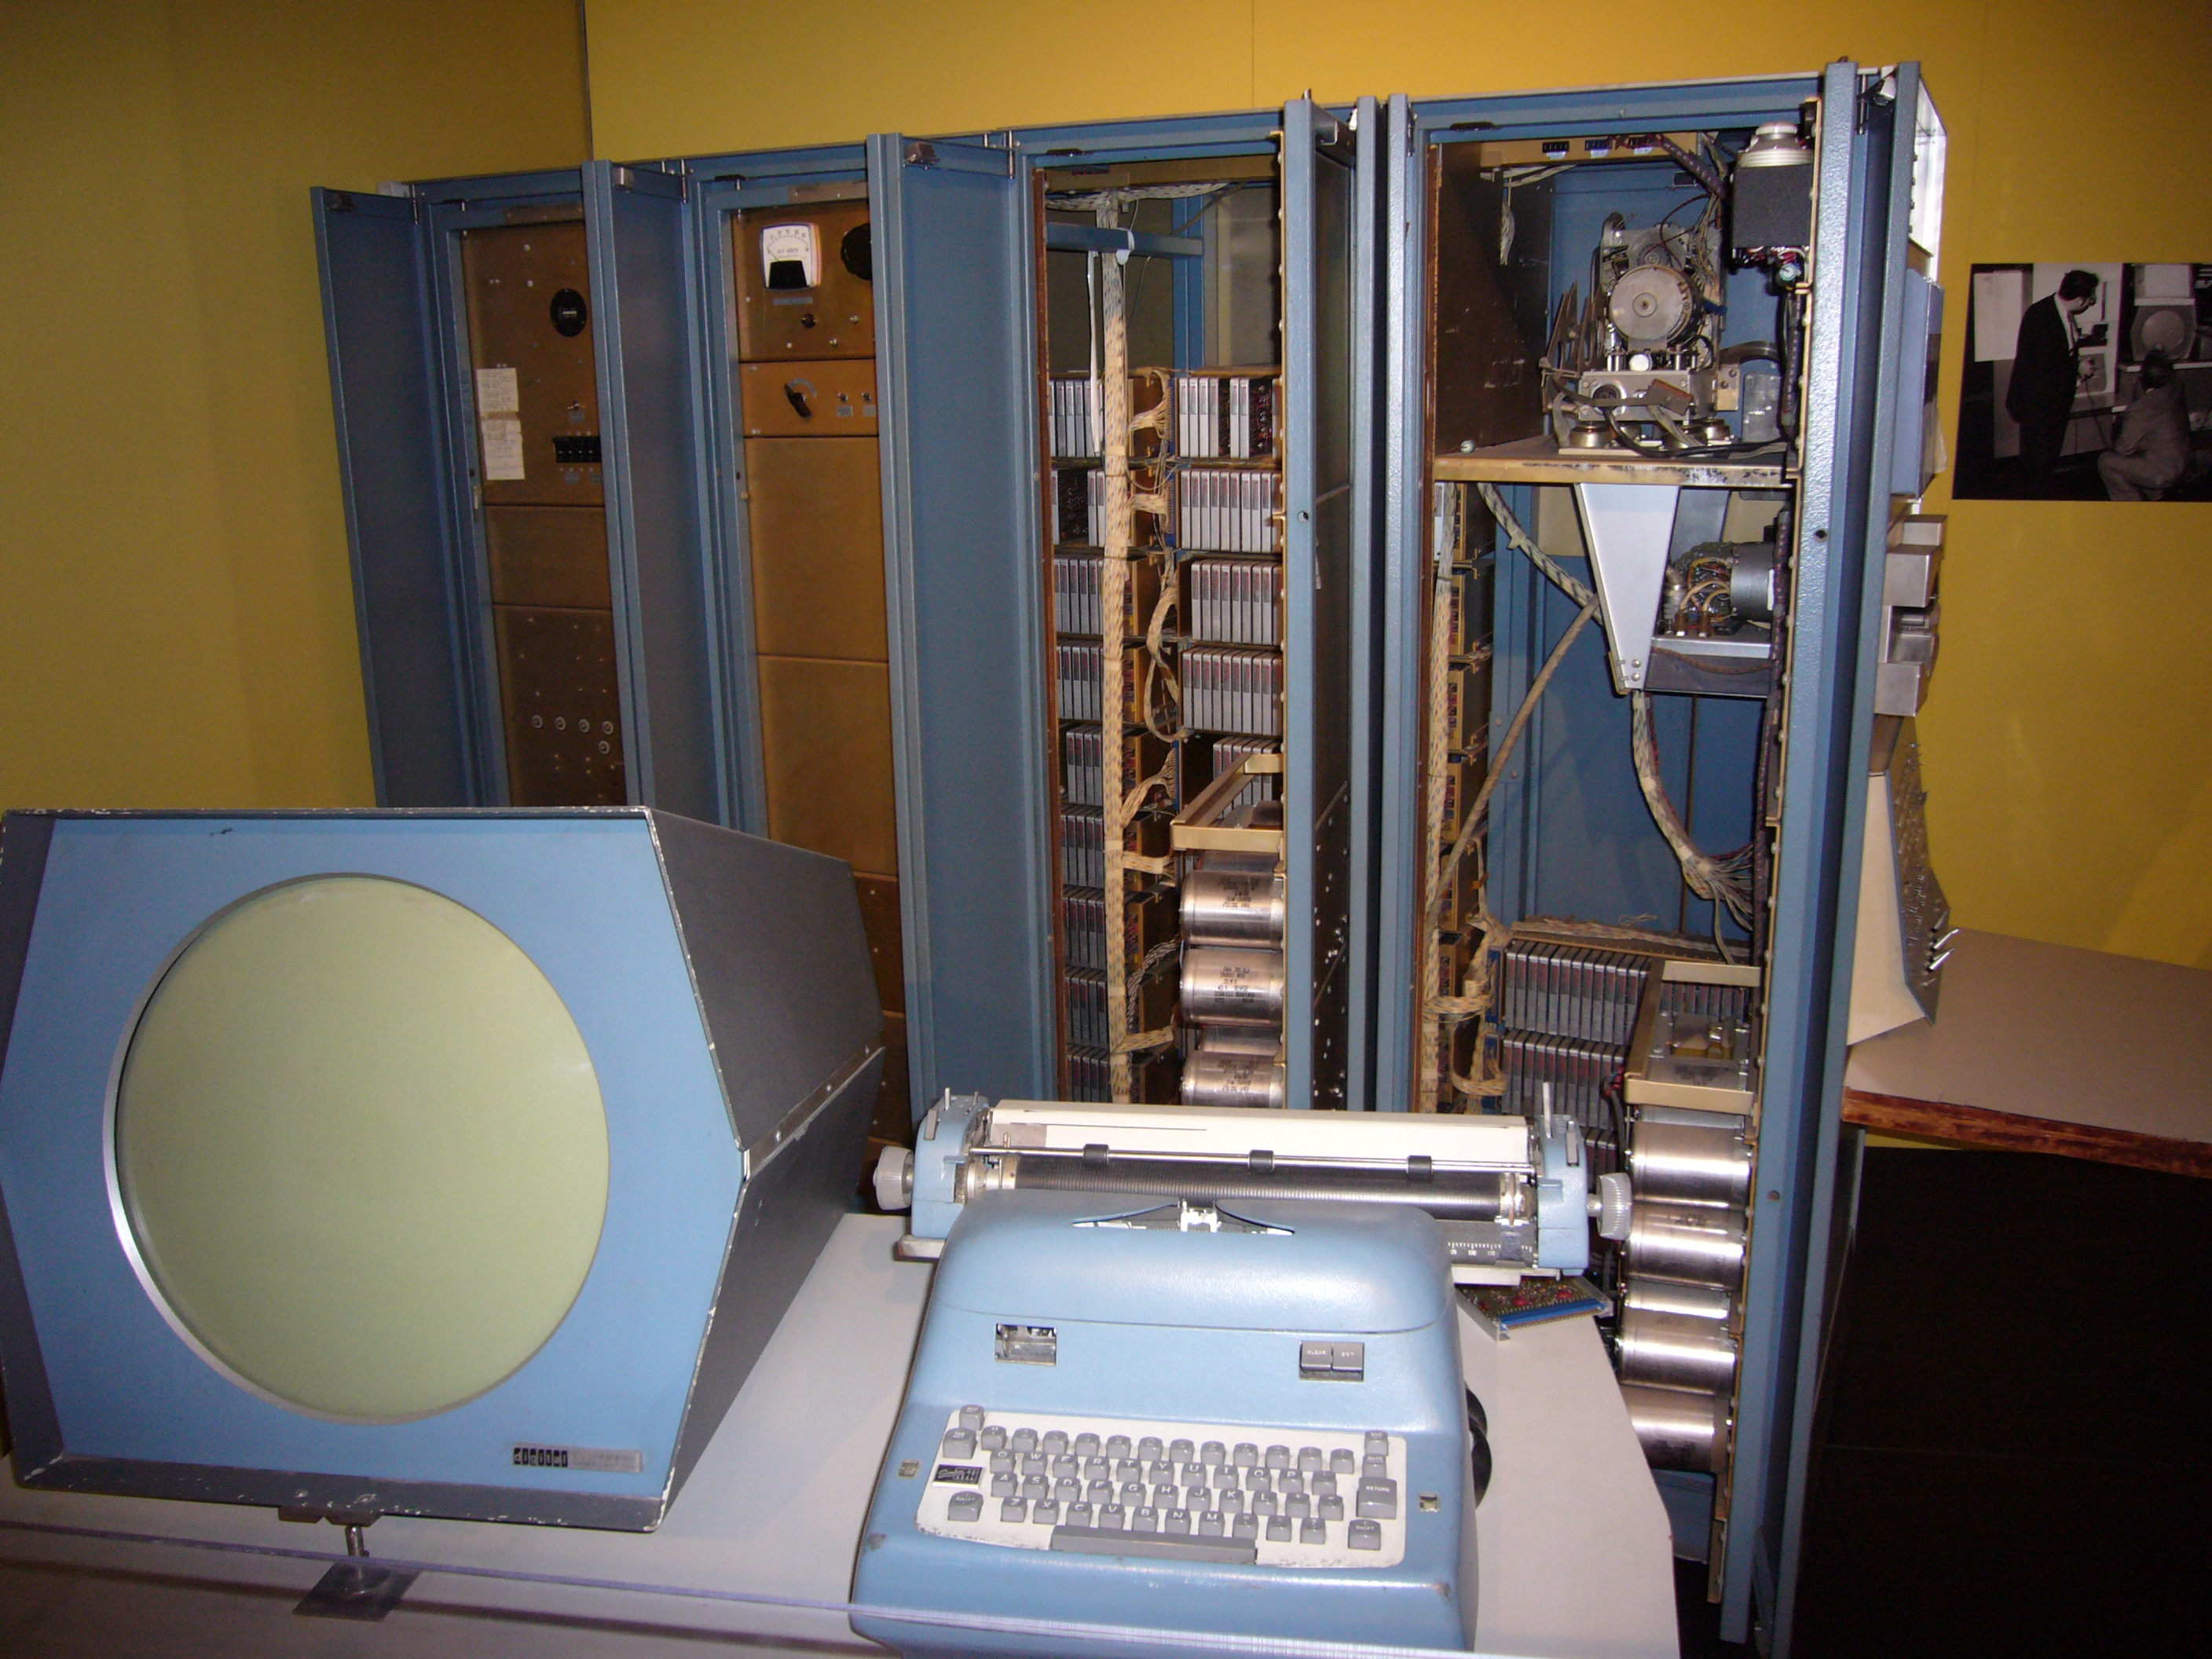
\includegraphics[width=0.7\textwidth]{media/Historia/Wikimedia_PDP-1.jpeg}
		    \caption{Fuente: Matthew Hutchinson - Flickr, Ordenador PDP-1.} %% Wikipedia https://es.wikipedia.org/wiki/PDP-1
	    	\label{fig:pdp1}
		\end{figure}
		%% Insertar imganes de computadoras
		
		Aún estaba lejos de terminar la década de 1960 y los circuitos integrados comenzaban a aparecer a la par de que desarrollos como la familia
		de computadoras \textit{System/360} de IBM empezaban a ocupar aún más velocidad y reducir su espacio para poder alcanzar un mercado más grande que aún era
		muy reducido en está generación\cite{oregan_brief_2012}. La era de las grandes computadoras que ocupaban toda una habitación se empezaba a ver desplazada apenas 10 
		años después de que 	
		empezara, y los continuos desarrollos de nuevas computadoras y de nuevas compañías sólo estaban empezando.
				
	\section{Más allá de los laboratorios}
		
		\subsection{Computadoras más compactas}
		

		El termino \textit{computadora}	era cada vez más recurrente en universidades y empresas, pero sólo aquellas con un alto presupuesto se podían
		dar el lujo de tener un mainframe en su oficina. Con la intención de aumentar el mercado algunas compañías estaban trabajando en productos
		comerciales que estuvieran al alcance de más entidades, el paso más relevante que se daría en la década de 1960 y marcaría el inicio de la tercera generación
		de computadoras lograba precisamente eso. El \textbf{circuito integrado} marcaría la siguiente gran revolución en la computación, inventado por
		Jack Kilby tuvo su primera demostración practica en 1958; un microchip de silicona(germanio en su invención) que permitía integrar
		en un mismo y diminuto chip docenas de transistores(u otros componentes eléctricos). Esto permitió tener computadoras más baratas, pequeñas y rápidas con una potencia 
		de procesamiento más
		alta. La historia detrás de esté invento es fascinante, fue tan importante que le permitió a su creador ganar el premio
		nobel de física en el año 2000, y por su puesto marco el inicio de una era de computadoras que podían salir de los laboratorios\cite{null_essentials_2003}.
		
		
		El siguiente paso a los \textit{mainframes} fueron las \textit{minicomputadoras}, que por su espacio podían caber en un auto(fig.\ref{fig:pdp8}),
		el termino podría parecer un poco antintuitivo para el lector del siglo 21 dado que las computadoras de la época son varias veces más pequeñas, pero
		para ese momento habían pasado de ocupar todo un cuarto para una computadora a sólo utilizar un escritorio. Una de las primeras, y la primera
		exitosa comercialmente, fue la \textbf{PDP-8(Programmed Data Processor -8)} creada en 1965 por ``\textit{Digital Equipment Corporation}, con un precio
		de 18,500 dólares fue todo un éxito en el mercado por la potencia que tenía contra su precio, que incluso era mucho más bajo que los precios de la serie
		\textit{System/360} de IBM, una línea de computadoras desarrollada con la intención de que todas fueran compatibles y que ya contaban con circuitos
		integrados\cite{null_essentials_2003}. En ese tiempo ``\textit{HP}'' empieza a sonar cada vez más fuerte en el mercado, y en 1966 lanza su primer computadora, la ``\textit{HP 2116A}
		que ya contaba con circuitos integrados para realizar las operaciones, era el momento dónde todas las empresas estaban sustituyendo sus
		transistores pro circuitos integrados, con esto cada vez más empresas de otros giros podían tener acceso a una computadora que 
		ayudará en sus operaciones diarias\cite{computer_history_museum_computers_nodate}.
		
		Una de las computadoras más pequeñas del momento fue la \textit{Apolo Guidance Computer(AGC)}, computadora diseñada específicamente para el viaje
		de la nave Apolo 11  a la luna y en la que lograron reducir el tamaño de ``7 refrigeradores'' a una computadora compacta que pesaba solo 70 libras.
 		La terminaron en 1968 y fue todo un hito en la ingeniería del momento, logro realizado por un equipo especializado del MIT que fue buscado
 		por el gobierno de Estados Unidos para completar una de las tareas más importantes para el despegue del Apolo\cite{computer_history_museum_computers_nodate}.
		
		\begin{figure}
		    \centering
		    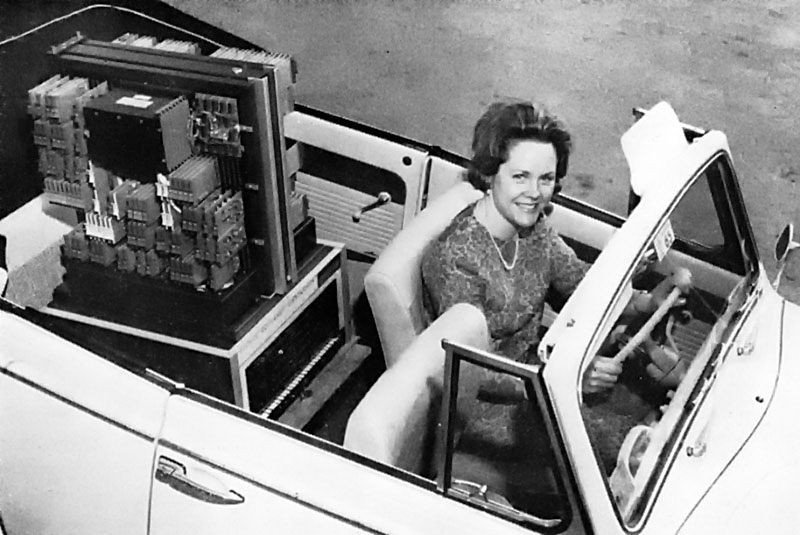
\includegraphics[width=0.7\textwidth]{media/Historia/CHM_computers_1964.pdp8.jpg}
		    \caption{Fuente:Computer History Museum, Ordenador PDP-8 en un automóvil.} %% Wikipedia https://es.wikipedia.org/wiki/PDP-1
	    	\label{fig:pdp8}
		\end{figure}
		
		La tercera generación también fue un punto de inflexión para los sistemas operativos y los lenguajes de programación, que en los principios
		ni siquiera eran considerados como temas realmente relevantes, el hardware primaba sobre cualquier avance en software, pero en está época
		los cambios y la importancia del software empiezan a ser cada vez más fuertes\cite{tanenbaum_modern_2002}.
		
		El final de la tercera generación llegaría con la invención del \textbf{microprocesador}, un sólo chip que podía contener miles de circuitos integrados,
		pero que no se detenía ahí, podía contener todos los componentes eléctricos de las computadoras, podías tener la unidad central de procesamiento(CPU por sus
		siglas en inglés) en la palma de tu mano. La primer microcomputadora\footnote{Se puede usar como sinónimo de computadora personal y hace alusión a que usaban microprocesadores.} exitosa y funcional
		fue la \textit{Altair 8800},desarrollada por la empresa MITS, venía en un kit para que los aficionados la pudieran armar; Contaba
		con el microprocesador \textit{Intel 8080}, era del tamaño de una caja, contaba con 256 bytes de memoria y costaba menos de 400 dólares, el cambio
		era gigante, pasaban de ser artefactos que sólo las grandes corporaciones podían adquirir a algo que una persona común con recursos suficientes
		podía comprar, no estaba al alcance de todos, pero ya estaba al alcance de muchas personas. Le seguirían las fas famosas \textit{Apple I}
		y \textit{Apple II} poco tiempo después, y en 1981 IBM introduciría su \textit{IBM PC(Personal Computer)}\cite{null_essentials_2003}.

		
		\clearpage
		\subsection{Lenguajes de programación}
		
		Hablar de los lenguajes de programación requeriría un libro completo para abarcar su historia y evolución, desde el uso de los algoritmos
		para resolver problemas, hasta la creación de ``lenguajes formales'' que funcionan de intermediario entre las personas y las maquinas. Pero
		en esta sección quiero abordar un breve repaso histórico sobre esté aspecto fundamental cuando hablamos de computadoras, y es que tales lenguajes
		son la forma en que nos ''comunicamos`` con estos aparatos para dar resolución a los problemas computacionales que tenemos.
		
		Para ser más claros debemos definir lo que es un algoritmo, que informalmente lo podemos definir como una colección de instrucciones simples para
		resolver alguna tarea, está definición nos sirve lo suficiente para entender el rol que tienen en la programación, una definición más formal es
		dada en la tesis de Church-Turing, que es la antesala de la teoría de la computación\cite{sipser_introduction_2013}. Siguiendo la definición informal
		podemos darnos cuenta de que esa ``colección'' es justo lo que se necesita para indicarle a una computadora lo que tiene que realizar, el único
		detalle está en que hay que traducirla de lenguaje humano a uno que la maquina entienda.
		
		La comunicación, entendiéndose como la forma de traducir instrucciones, entre humanos y computadoras está		
		completamente ligada al desarrollo del hardware computacional, a medida que las computadoras se volvían más potentes se requería
		una forma más sencilla de traducir los problemas de lenguaje humano a lo que se conoce como \textit{lenguaje maquina}, que son las instrucciones en números
		binarios o decimales dependiendo la arquitectura que sea la maquina(las actuales son en su mayoría binaría). Por ejemplo para programar las primeras maquinas
		de propósito especifico como ENIAC o Colossus se usaban enchufes y cables para poder definir patrones en lenguaje maquina que daban la instrucción a la computadora de 	
		hacer una tarea en especifico\cite[p. 8]{tanenbaum_modern_2002} \footnote{Un ejemplo de como funcionaban las computadoras se puede ver en el siguiente vídeo: \emph{ 
		Colossus \& Other Early Computers}, [Vídeo], \url{https://www.youtube.com/watch?v=KkSxC9pFGZs} }. 
		
		Pero a medida que las computadoras fueron aumentando su complejidad y podían resolver problemas más complejos el traducir estos problemas más complejos
		a lenguaje maquina se volvía una tarea muy ardua, incluso con la mejora de la inclusión de las tarjetas perforadas para programar a principios de los
		años 50 llevar un problema a lenguaje maquina era una tarea en la que se perdía mucho tiempo. De ahí que empiezan a surgir ideas para hacer esté proceso
		más amigable con el usuario, ahí se empieza a gestar la idea del ``lenguaje ensamblador'', que en la definición que da \cite{salomon_assemblers_1992} nos
		dice:
		
		\begin{quote}
			\emph{Un ensamblador es un traductor que traduce instrucciones de origen(en lenguaje simbólico) a instrucciones de destino(en lenguaje maquina), uno a uno.}
		\end{quote}
		
		Es decir que se crea un lenguaje simbólico para poder sustituir las instrucciones en bruto en código maquina, este lenguaje por supuesto necesitará
		de una traducción para esas instrucciones. Aunque en las versiones más arcaicas del uso de esté tipo de lenguaje para programar más bien se usaba
		para describir un problema de forma más entendible para los humanos que después manualmente se traducía por otras personas a lenguaje maquina.
		En el vídeo \cite{maurice_vincent_wilkes_edsac_1976} creado por el mismo Maurice Wilkes, creador de la EDSAC, nos muestra el proceso de programación que se
		seguía en la EDSAC, el cuál tenía un lenguaje simbólico para definir los problemas, pero aún así se requería de una traducción manual para llevarlo
		a ejecución en la EDSAC. El siguiente paso en el uso del lenguaje simbólico lo podemos ver en la misma EDSAC por que a pesar de que mencione
		que se tenía que hacer una traducción manual había un programa llamado \textit{Initial Orders} que se cargaba de inicio en la maquina, que funcionaba como
		un traductor o lo que hoy llamaríamos \textit{ensamblador arcaico} por que traducía algunos códigos muy específicos que facilitaban la programación
		\cite{salomon_assemblers_1992,richards_edsac_nodate}.
		
		Los siguientes pasos en facilitar la programación fueron la creación de ensambladores más en forma para que el programador sólo necesitara
		escribir el programa en lenguaje simbólico y el ensamblador pudiera traducirlo a lenguaje maquina. Ya en 1953 la IBM 650 incluía un ensamblador
		llamado \textit{SOAP(Symbolic Optimizer and Assembly Program)}, sólo 7 años después de la UNIVAC, esté programa daba mucha más facilidad a los programadores
		para desarrollar sus problemas en un lenguaje más amigable\cite{salomon_assemblers_1992}.
		
		Quizá todos estos avances para el programador actual parezcan muy simples, pero fueron verdaderas innovaciones que buscaban que el programador
		destinara más tiempo a resolver problemas y menos a traducir códigos. Es en está época, mediados de los años 50 e inicios de los años 60 la idea
		era ir más allá de los lenguajes de ensamblador, que si bien eran una mejora aún se tenía que seguir prácticamente la misma lógica para programar. con
		la facilidad de no tener que hacerlo únicamente con números claro está, así que el siguiente avance lógico serían los \textit{lenguajes de alto nivel}. La idea
		de estos lenguajes era facilitar la lógica de programación, que el programador ya no se tuviera que preocupar por direcciones de memoria y se centrara
		en otros aspectos más sustanciales, como la optimización y calidad de su programa. A estos lenguajes se les puede llamar la \textbf{tercera generación}
		de lenguajes de programación, antecedidos por el lenguaje maquina y el ensamblador como primera y segunda generación respectivamente\cite{oregan_brief_2012}.
		
		Se debe hacer mención especial a \textbf{Plankalk\"{u}l},que traducido significa algo así como ``calculo de programas'', el primer lenguaje de programación de alto 
		nivel, desarrollado por Konrad Zuse en 1946 para su serie
		de computadoras \textit{Z}, incluía estructuras de datos, álgebra booleana y condicionales, entre otros aspectos que lo asemejan demasiado a lenguajes más modernos, a
		lenguajes que en el mundo ``occidental'' no llegarían hasta mediados de los años 50. Lamentablemente esté y sus demás descubrimientos quedaron sepultados por mucho 
		tiempo a causa de la segunda guerra mundial\cite{oregan_brief_2012}\footnote{En el vídeo: \emph{Computer History: Dr. Konrad Zuse, Computer Pioneer and the Z 
		Computers (Z3)}, \url{https://www.youtube.com/watch?v=6GSZQ9g-jiY} se puede conocer un poco más de esté lenguaje y su creador.}.
		
		No sería hasta mediados de los años 50, en la era de los mainframes y de las primeras minicomputadoras, que los primeros lenguajes de programación
		de alto nivel comenzarían a surgir. Dos gigantes que aún existen hoy en día nacieron en esa época, \textbf{FORTRAN}(Formula Translating System) desarrollado por IBM y
		\textbf{COBOL}(Common Bussines-Oriented Language) desarrollado por un el comité CODASYL; El primero orientado principalmente al sector científico que usaba
		las computadoras y el segundo más enfocado en los negocios y las empresas que necesitaban formas más amigables y óptimas de programar\cite{oregan_brief_2012}.
		%% Sección para los compiladores		
		
		
		En los años siguientes el desarrollo de nuevos lenguajes de programación con diferentes enfoques continuo, desde Pascal, C y Basic, pasando por otros más modernos 
		como Python y Java, junto a muchos más que
		se han continuado desarrollando con una idea en común, facilitar la programación, que el programador no se torture buscando formas de transmitir sus
		ideas a la maquina y que se enfoque en diseñar los algoritmos correctos para resolver sus problemas.
		
		%% Falta mencionar lo de los compiladores


		\clearpage
		\subsection{Sistemas operativos y los cambios en el paradigma de programación}
		
		Posiblemente la palabra \textbf{Sistema Operativo} le resulte muy común al lector contemporáneo, prácticamente todos los que tenemos contacto con
		la tecnología sabemos que el celular que usamos usa un sistema operativo llamado ``Android'' o ``IOS'', que nuestra computadora seguramente tiene
		un sistema llamado ``Windows´´ o si somos muy aficionados a los sistemas operativos quizá tengamos ``GNU/Linux''. Tal como los lenguajes
		de alto nivel los sistemas operativos no estaban presentes cuando se crearon las primeras computadoras, estos aparecieron años más tarde cuando
		las tareas se volvieron más complejas, con maquinas más potentes y con usuarios que querían un trabajo menos estresante. Y aún así un sistema operativo
		reconocible por alguien del siglo 21 aparecería hasta los años 80 por ejemplo con, el ahora legendario, \textbf{MS-DOS} para las computadoras de IBM y potencialmente
		para cualquier empresa que pudiese pagar por su licencia.
		
		Pero ¿que es un sistema operativo?, la respuesta no es simple, pero para explorar su evolución podemos entender a un sistema operativo como un programa especial 
		dentro de la maquina que realiza dos tareas principales; ser una conexión entre los demás programas y el hardware del ordenador, 
		y gestionar los recursos del hardware\cite{tanenbaum_modern_2002}.
		
		En el libro \cite{tanenbaum_modern_2002} nos presenta la evolución de los sistemas operativos siguiendo
		el esquema de las generaciones de computadoras, empezando en
		la \textbf{primera generación}(1945-1955) con la primera de las computadoras y la prácticamente inexistencia de los sistemas operativos o algo cercano en ellas,
		dado que como vimos en la sección anterior la programación era básicamente en lenguaje maquina y quizá en algo cercano aun ensamblador como
		lo fue ``Initial Orders''. Y aunque no fue muy relevante esa época para los sistemas operativos si nos dejo, justamente en ``initial orders'', un ejemplo
		muy temprano de lo que puede hacer un \textit{loader}, que es básicamente un programa que carga programas en la memoria, lo cuál no es una tarea sencilla,
		puesto que debe llevar cada instrucción a su correspondiente lugar en memoria, por ende, entre más compleja es la maquina más compleja
		será la tarea del ``loader''\cite{salomon_assemblers_1992}.
		
		La \textbf{segunda generación}(1955-1965) que se encuentra en la época de los mainframes y de los primeros lenguajes de alto nivel nos deja
		los sistemas \textbf{batch} como ancestros más directos de los sistemas operativos. En está época ya se tenían a más usuarios trabajando en más maquinas, por
		lo que se requería de un nivel de servicio cada vez más alto, el que cada usuario fuese con una maquina, dejará su programa y esperara a que le diera
		respuesta el operador era poco eficiente, la idea que generalmente se adopto para resolver esto fueron los sistemas batch. Básicamente es una forma de trabajo
		en la que se colecta un conjunto de \textit{jobs}(un conjunto de programas usualmente de un usuario) para que una o varias maquinas los procesen, sin intervención 
		humana, y se entreguen los resultados a los usuarios una vez se hayan terminado de ejecutar. En este flujo tienen relevancia, además de los programadores,
		los operadores que llevaban esos \textit{jobs} y cargaban en las maquinas, que además necesitaban cargar los ``loaders'' cuando eran requeridos y los
		compiladores si se había trabajado en algún lenguaje de alto nivel; entre los programas especiales como los ``loaders'' y los operadores hacían
		el trabajo que hoy se asocia a los sistemas operativos.
		
		Para esté punto ya tenemos una necesidad, un programa que administre los recursos de la maquina,  y hacía la \textbf{tercera generación} de computadoras(1965-1980)
		se vislumbraría la otra. Había dos ramas en la construcción de las computadoras, las maquinas con un enorme poder computacional(para su época) enfocadas
		en cálculos científicos, y las computadoras comerciales que tenían un mercado en las empresas. La aproximación que dio IBM para solucionar esto
		fue crear una familia de computadores que tuvieran ciertas características en común a nivel de hardware, con un sistema operativo común llamado
		\textbf{OS/360}, el cuál tenía la intención de funcionar en todas las computadoras de está familia y funcionando como enlace para los demás programas y el software
		de forma que no se tuviera que programar de una forma totalmente distinta entre una maquina y otra. El problema con esté sistema operativo, es que para funcionar
		tanto en computadoras orientadas a hacer pronósticos del clima y otros complicados cálculos, así como ejecutar operaciones como imprimir información
		para ambientes más comerciales hacían de este sistema operativo un programa realmente complejo, construido con millones de lineas en lenguaje ensamblador
		era realmente difícil darle mantenimiento. Pero es que para cumplir con todos los requerimientos de un sistema operativo es inevitable pensar en un programa
		de millones de líneas de código, los libros de \cite{tanenbaum_modern_2002} y \cite{silberschatz_operating_2009} muestran en su portada, con un toque de sátira,
		dos formas diferentes que un sistema operativo es un programa extremadamente complejo y que controla muchas actividades de la maquina; Silberschatz lo muestra
		con la clásica portada de dinosaurios haciendo referencia al libro que escribió Fred Brooks, uno de los diseñadores de de OS/360 y Tanenbaum con un circo que
		tiene una cantidad muy grande de participantes que son parte del sistema operativo.
		
		Ahora que se tenía un sistema operativo que agilizaba bastante las tareas, a pesar los problemas que tenía, surgieron otras formas de procesar
		los programas para aumentar la eficiencia, ahora se podía conseguir la \textbf{concurrencia}. La concurrencia no es más que la ejecución de varios
		procesos en ``simultaneo'', es decir que se ejecuta parte de un proceso A y luego parte de un proceso B, buscando la eficiencia y que ambos usuarios obtengan
		sus resultados de forma eficiente sin retrasar al otro. Particularmente cobro mucha notoriedad una técnica llamada ``multiprogramming'', ``multitasking'',
		o ``multiprogramación'', lo que buscaba es explotar al máximo los ``tiempos muertos'' generalmente causados cuando el ordenador esperaba alguna instrucción por
		parte del usuario, en maquinas comerciales alrededor del 80\% o 90\% del tiempo era usado en esto, por lo que con  la multiprogramación se le da tiempo
		de procesamiento a otro programa que este en espera. Está forma de computación es la que actualmente se utiliza en las computadoras que tenemos, dando
		la sensación de que todos los programas que se ejecutan están ejecutándose al mismo tiempo, aunque en aquellos tiempos el procesamiento no era
		tan rápido para pensar esto, la comodidad para los usuarios al momento de usar computadoras mejoro mucho. Cabe destacar que las computadoras actuales tienen
		más que solo computo concurrente, como por ejemplo computo paralelo, pero eso será revisado más adelante.
		
		%%Año de los sitemas 360
		
		En este contexto hay otra variante de la multiprogramación que es importante mencionar, el \textbf{timesharing}, aunque dejo de tener relevancia cuando
		las computadoras se volvieron tan potentes como para tener una por persona, pero que dejo muchas enseñanzas que se siguen aplicando. El concepto busca
		la concurrencia al igual que la multiprogramación, pero la diferencia es que la segunda en esos momentos estaba principalmente implantada para
		sistemas batch, lo que buscaba el timesharing es proveer a los usuarios una respuesta más inmediata, que por ejemplo les ayudara en la tarea de
	    debbugear\footnote{Es una palabra proveniente del idioma inglés que se usa para expresar que se hacen pruebas para detectar errores en el algoritmo} sus programas. 
	    De hecho su invención vino desde antes del uso de la multiprogramación, en 1961 fue presentado el \textbf{CTSS(Compatible Time-Sharing System)}, desarrollado
	    en el M.I.T., el problema que tuvo es que no se contaba con el hardware necesario para uso en masa, y seguridad de protección suficiente para sus usuarios,
	    en el sentido de aislar a los diferentes usuarios involucrados por ejemplo. Pero la popularización del time sharing en la tercera generación de computadoras
	    se dio, y llego tan lejos que el MIT, Bell Labs y GE intentaron construir un sistema operativo llamado \textbf{MULTICS} que funcionara sobre maquinas conectadas por 
	    la red eléctrica para soportar cientos de usuarios, por supuesto la tarea era demasiado ambiciosa para su tiempo, pero aunque al final GE y Bell Labs
	    salieron del proyecto el sistema operativo termino funcionando de la mano del MIT, de hecho tuvo una gran influencia para el desarrollo de \textbf{UNIX} que
	    a su vez es una gran influencia para sistemas como GNU/Linux, macOS, y FreeBSD. Quizá el concepto de tieme-sharing como se conocía en esa época no llego
	    a nuestros días, pero el \textbf{Cloud Computing} es una clara evolución, con maquinas miles de veces más potentes para un uso masivo de miles de
	    usuarios\cite{tanenbaum_modern_2002}.
		
		Precisamente esté sistema operativo, MULTICS, en 1969 era capaz de trabajar con múltiples procesadores en \textbf{paralelo}, un concepto que
		no puede faltar en las computadoras actuales\cite[p. 899]{silberschatz_operating_2009}. Esto fue un avance importante
		en la construcción de computadoras cada vez más potentes, por que al añadir más procesadores puedes conseguir computadoras más potentes, pero necesitas de un sistema 	
		que pueda manejar estos procesadores y aprovecharlos de forma eficiente. Cabe aclarar que no es la única forma de paralelismo, puede haber paralelismo en
		los datos, o bien en las instrucciones, incluso paralelismo a nivel instrucción, entre muchos otros\cite{null_mariesim_2003}; haciendo énfasis en que está tesis se 
		centrará en	el paralelismo de múltiples procesadores.
		
		Pero sus inicios no fueron fáciles, requerían de hardware muy especializado para realmente ser útiles, realmente no hay muchos casos documentados
		de computadoras o sistemas paralelos en la tercera generación de computadoras, la ILLIAC IV es un ejemplo de computadora con
		una arquitectura y un sistema que podían explotar los beneficios del paralelismo, de hecho por la potencia que logro se dice que es la primer supercomputadora. Aunque 
		culmino su desarrollo a mediados de los años 70, tuvo muchos problemas
		principalmente relacionados al hardware de la época, pero sus logros no faltaron tampoco y por algo es recordada aún hoy en día como una de las pioneras en el
		mundo del paralelismo\cite{hord_illiac_1982}.
		
		Para las computadoras personales de la \textbf{cuarta generación} tampoco fue una adaptación inmediata, por ejemplo las primeras computadoras de IBM y Apple no tenían
		múltiples procesadores o alguna arquitectura enfocada al paralelismo, no fue hasta los años de 1990 y principios de los 2000 que el ascenso de las computadoras con 	
		múltiples procesadores llegaría.
		A pesar de que las ideas de arquitecturas paralelas como los multiprocesadores estaban ahí desde décadas antes, e incluso había varías implementaciones,
		especialmente en supercomputadoras, aún faltaba que las computadoras evolucionaran tanto a nivel hardware como software para 
		volverse una opción realista para las computadoras, puesto que no solo necesitas múltiples procesadores(en el caso de dicha arquitectura) sino un sistema operativo 	
		que pueda organizar los recursos de manera eficiente para lograr que sea realmente útil la arquitectura\cite{computer_history_museum_computers_nodate}.
		
		
		\clearpage		
		
		\subsection{Creación de los modelos didácticos de enseñanza}
		%El como nace el modelo para dar claridad a los trabajadores de ATT, razones de las computadoras personales
		% Imagenes de como se programaba
		
		Estamos a mediados de los años 60, época del estreno de \textit{Star Trek} que empezaba a maravillar a las personas con su ciencia ficción  y sus
		computadoras que podían resolver cualquier problema, poco antes del primer viaje a la luna(realizado en el Apollo 11) y sobretodo
		en un tiempo en que el desarrollo tecnológico sólo iba creciendo. Como ya leímos en secciones
		anteriores
		es la época dónde las computadoras empiezan a ser más pequeñas, curiosamente a computadoras como la \textit{PDP-1} y la serie de computadoras que detono les llamaban 
		``minicomputadoras'' dado que la reducción de tamaño comparada con otras como la legendaria \textit{ENIAC} era enorme, una época dónde
		los sistemas operativos aún no llegaban al uso masivo y los primeros lenguajes de alto nivel estaban apareciendo entre los usuarios. Uno de los 
		problemas para esté tiempo era claramente el tener que explicar
		a los usuarios el funcionamiento de las computadoras cuando estos no habían visto una computadora en su vida, y la primera vez que la veían era para usarla,
		es algo bastante complejo, así que se buscaron alternativas a la pura teoría que pudieran hacer de este un mejor proceso, así fue que varias empresas 
		y universidades(de estados unidos principalmente) empezaron a desarrollar modelos didácticos de enseñanza de las computadoras que no requiriesen de una computadora 
		real, y es que aunque había universidades con bastante prestigio como el MIT que tenían algunos modelos de computadoras para la investigación, era difícil
		el acceso para los alumnos, por no decir imposible\cite[p. 71]{ceruzzi_computing_2012}. Una de esas compañías era \textbf{Bell Telephone 
		Laboratories} mejor conocido como \textit{Bell Labs}, en aquellos tiempos era un centro de trabajo y de investigación muy prestigioso, y parte de la
		poderosa \textit{American Telephone and Telegraph} que a pesar de que su negocio
		principal eran los teléfonos, tenía un área de investigación dedicada al desarrollo de nuevas tecnologías; fue en los laboratorios bell dónde se inventó el 		
		transistor,
		que dio un cambio total a la concepción de las computadoras dada la cantidad de espacio que  ahorrar sin perder la potencia de computo, e incluso mejorarla
		comparada a sus antecesoras las bombas de vacío\cite[p. 161]{isaacson_innovators_2014}. Pero \textit{Bell Labs} no sólo se dedicaba a la investigación,
		también tenía una sección dedicada a la enseñanza, en la cuál se asociaba con universidades para repartir materiales entre ellas y kits de aprendizaje de diversos
		temas relacionados a las investigaciones de los laboratorios, por ejemplo posterior a la invención del transistor sacaron un documental junto
		con un kit electrónico que incluía un pequeño transistor para que los estudiantes pudieran estudiar con aparatos tecnológicos reales y aprender
		de los ``expertos'' su funcionamiento, los documentales además estaban dirigidos a publico no experto en la nueva área de las computadoras y por ende
		eran bastante claros, hoy en día el canal de You Tube \textit{AT\&T Tech Channel}(canal de la empresa) recopila muchos de estos documentales, un ejemplo es el 
		documental del transistor \cite{att_tech_channel_transistor_2015}.
		
		%% Se podría agregar la definición de modelo
		
		Estás acciones no eran altruismo para Bell Labs, pero aún así a los estudiantes de las 
		escuelas dónde
		llegaban estos \textit{kits} les era de gran ayuda, hoy en día prácticamente todo lo podemos investigar en internet, pero en aquel tiempo se dependía de las
		bibliotecas y algún apoyo como el de Bell Labs.
		
		Así fue como en 1968 laboratorios Bell lanza un kit(una caja de cartón), acompañado con un vídeo llamado \textbf{Thinking Machines}, el
		cuál se puede encontrar en youtube \cite{att_tech_channel_att_2012} ,en el cuál narran
		a través de la pregunta ``¿las computadoras piensan'' la lógica que siguen las computadoras para resolver las tareas que se les daban y los funcionamientos
		internos que tienen para solucionar los problemas que les asignamos. En la caja de cartón venía el manual de instrucciones 
		\cite{david_hegelbarger_instruction_1968} y unas hojas de papel como se ve en la figura \ref{fig:Kit_CARDIAC}, con estos elementos el 
		estudiante podía empezar la construcción de su ``propia computadora de papel'', el resultado se puede ver en la figura \ref{fig:CARDIAC_Construida} 
		\cite{megardi_cardiac_nodate}.
		A la derecha de la imagen tenemos el espacio de memoria con un 001 al inicio y un ``8--'' al final como apartados de memoria reservada, a la izquierda
		está la unidad de procesamiento central, el lugar dónde llegan los datos desde la memoria y se realizan las operaciones aritméticas y lógicas
		que se depositan en el acumulador.
		
		\begin{figure}[h]
			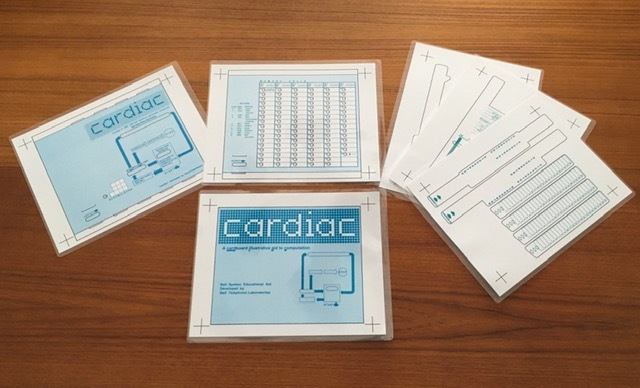
\includegraphics[scale=0.3]{media/CARDIAC_Paper/paper1.jpg}
			\caption{Kit de CARDIAC abierto}
			\label{fig:Kit_CARDIAC}
		\end{figure}
		
		\begin{figure}[h]
			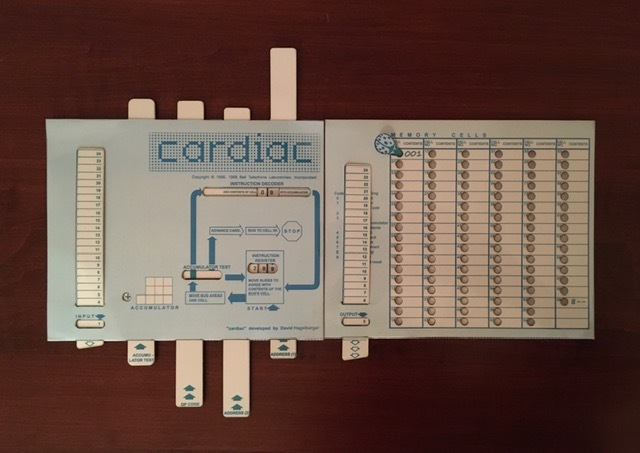
\includegraphics[scale=0.3]{media/CARDIAC_Paper/Construida.jpg}
			\caption{CARDIAC construida}
			\label{fig:CARDIAC_Construida}
		\end{figure}
		
		
		Con esta estructura de papel es posible realizar las operaciones básicas que hace una computadora a la vez que puedes ir viendo el proceso que llevan
		los datos desde la entrada(teclado o una tarjeta perforada) hacía la memoria principal y el flujo que sigue la ``maquina'' para ejecutar
		las instrucciones que están en la memoria y diferenciarlas de los datos, así como la interpretación de esas instrucciones, su procesamiento lógico y los
		cálculos aritméticos, hasta que llegan al acumulador y de ahí según lo que dicten las instrucciones se puede seguir trabajando con
		esos datos en el acumulador o guardarlos en memoria para su posterior ``impresión'' fuera de la memoria. Este proceso es, muy a grandes rasgos y muy simplificado
		lo que realizan nuestras computadoras hoy en día(con varias mejoras), pero que nosotros no vemos, sólo vemos los resultados, es por está situación que a nosotros
		como estudiantes del siglo 21 que ya contamos con una computadora a nuestro alcance, en mayor medida que en los años 60, nos puede ser de utilidad
		CARDIAC para razonar y analizar los procesos que se ejecutan en una computadora y entender su funcionamiento; quizá hoy en día un CARDIAC de papel
		no nos sea tan practico, pero el concepto si que lo es, y llevarlo a un entorno electrónico que nos de más potencia sin perder la esencia del modelo
		didáctico que es
		CARDIAC puede ser una gran ayuda para comprender como opera una computadora.

		\clearpage		

	
		\subsection{Actualidad de las computadoras}
		
		
		La evolución desde los años 80 hasta la actualidad ha sido sorprendente, es muy interesante leer o ver los comentarios de las personas que han interactuado
		con las computadoras en este lapso de tiempo y han sentido el cambio directamente en su trabajo diario, pasar de usar esos enormes mainframes
		llamados minicomputadoras, a esas pequeñas computadoras que hoy nos parecen más maquinas de escribir con una pantalla, y por supuesto a las 
		computadoras que tenemos en la palma de nuestra mano en forma de celulares o tabletas. Evidentemente si hacemos una comparación directa las diferencias
		son bastante claras, pero si nos vamos a los detalles, como hemos visto, hay muchos aspectos que conservan de sus antepasados, otros que incluso sólo
		han ``mejorado'', pero que el concepto sigue siendo el mismo. Como lo es el procesador que utiliza una maquina, o la misma arquitectura, que en su mayoría sigue la 
		arquitectura de Von Neumman o bien la que se ha vuelto muy popular con los teléfonos móviles, una versión moderna de la ya lejana
		arquitectura Harvard que viene en los procesadores ARM \cite[p. 109]{valvano_introduction_2017}. Y también hay cambios bastante notables, como el computo en la nube o 
		computo distribuido, que toma la 
		herencia del ahora innecesario time-sharing(por la potencia de las computadoras actuales), pero que toma el concepto base y lo lleva mucho más lejos de lo que siquiera 
		llegaron a pensar los creadores de los primeros modelos computacionales que incluían el tieme-sharing.
		
		Quizá las dos más grandes novedades de la computación moderna, los procesadores ARM y el computo en la nube, entre otros avances a nivel de hardware
		como los son las GPU o TPU, procesadores especializados para realizar operaciones matemáticas muy concretas, o a nivel de software como
		la inteligencia artificial y el \textit{blockchain} nos recuerdan que en el mundo de la computación nada es estático, y la evolución es continua.
		 

\chapter{Teoría de la computación} %¿Demasiado pretencioso el titulo?

	\section{Funcionamiento básico de las computadoras}   %% Se podría ampliar a partes más teoricas de automatas
		
		\subsection{Arquitectura Von Neumann}   
	
		\subsection{Sistema Operativo}   	

	\section{Modelos de computo}

		\subsection{Modelo concurrente}

		\subsection{Modelo paralelo}
	
		\subsection{Modelo distribuido}

\chapter{CARDIAC y su evolución}  %
	\section{Operaciones concurrentes}
	
		\subsection{Necesidad de un sistema operativo}
		
		\subsection{Mejoras necesarias en el Hardware}
		
		\subsection{Creación de una arquitectura concurrente}
	
	 \section{Evolución hacia el paralelismo}
	 
	 	\subsection{Hardware y sus necesidades actuales}
	 	
	 	
	 	\subsection{Arquitectura paralela E-CARDIAC PAR}


\chapter{Conclusiones}

\newpage

\selectlanguage{spanish}
	\bibliography{CARDIAC}
\selectlanguage{spanish}
	\bibliographystyle{apacite}

%\backmatter%@sglvgdor


\end{document}
